\documentclass[11pt,a4paper,titlepage]{report}

\usepackage[utf8]{inputenc}
\usepackage[T1]{fontenc}
\usepackage{lmodern}
\usepackage{geometry}
\geometry{top=1.0in, bottom=1.0in, left=1.0in, right=1.0in}
\usepackage{amsmath,amssymb,amsfonts,mathtools,bm}
\usepackage{graphicx}
\usepackage{booktabs}
\usepackage{microtype}
\usepackage{enumitem}
\usepackage{titlesec}
\usepackage{fancyhdr}
\usepackage{xcolor}
\usepackage[most]{tcolorbox}
\usepackage{hyperref}

\setlength{\headheight}{14.5pt}
\addtolength{\topmargin}{-2.5pt}

% Define color palette
\definecolor{DeepNavy}{RGB}{29, 53, 87}
\definecolor{SlateBlue}{RGB}{69, 123, 157}
\definecolor{LightIce}{RGB}{241, 250, 238}
\definecolor{CoralRed}{RGB}{230, 57, 70}
\definecolor{Charcoal}{RGB}{43, 45, 66}
\definecolor{BoxBg}{RGB}{248, 249, 250}

\hypersetup{
    colorlinks=true,
    linkcolor=DeepNavy,
    citecolor=SlateBlue,
    urlcolor=SlateBlue,
    pdfauthor={Doctoral Research Lab},
    pdftitle={Federated Foundation System Architecture and Theoretical Foundations}
}

% Header and Footer Styling
\pagestyle{fancy}
\fancyhf{}
\fancyhead[L]{\textcolor{DeepNavy}{\small\textsc{Federated Learning Architecture Manual}}}
\fancyhead[R]{\textcolor{Charcoal}{\small\textsc{Chapter \thechapter}}}
\fancyfoot[C]{\thepage}
\renewcommand{\headrulewidth}{0.5pt}
\renewcommand{\footrulewidth}{0pt}

% Title formats
\titleformat{\chapter}[display]
  {\normalfont\bfseries\color{DeepNavy}}
  {\Large\textsc{Chapter} \thechapter}{10pt}{\Huge}
\titlespacing*{\chapter}{0pt}{-20pt}{25pt}

% Custom TColorBoxes
\newtcolorbox{elevatorpitch}{
    colback=LightIce,
    colframe=DeepNavy,
    fonttitle=\bfseries\color{white},
    title=Advisor Elevator Pitch (30-Second Summary),
    boxrule=1.0pt,
    arc=4pt,
    top=8pt, bottom=8pt, left=10pt, right=10pt
}

\newtcolorbox{defenseqa}[1]{
    colback=BoxBg,
    colframe=SlateBlue,
    fonttitle=\bfseries\color{white},
    title=PhD Defense Hot Seat: #1,
    boxrule=1.0pt,
    arc=4pt,
    top=8pt, bottom=8pt, left=10pt, right=10pt
}

\newtcolorbox{mathfoundation}{
    colback=white,
    colframe=Charcoal,
    fonttitle=\bfseries\color{white},
    title=Mathematical Formulations and Optimization Objectives,
    boxrule=1.0pt,
    arc=4pt,
    top=8pt, bottom=8pt, left=10pt, right=10pt
}

\begin{document}

\begin{titlepage}
    \centering
    \vspace*{1.2cm}
    {\Huge \textbf{\textcolor{DeepNavy}{Federated Foundation System Architecture \& Theoretical Foundations}}}\\[0.5cm]
    {\Large \textsc{\textcolor{SlateBlue}{The Visual, Intuitive Field Guide}}}\\[1.2cm]

    \rule{0.85\textwidth}{1.5pt}\\[1.2cm]

    {\Large \textbf{\textcolor{Charcoal}{Clear Architecture • Rigorous Math • Confident Defense}}}\\[0.4cm]
    \textit{Demystifying distributed learning, JAX/Flax engines, privacy, and compression}\\[2.2cm]

    \begin{minipage}{0.48\textwidth}
        \begin{flushleft} \large
            \textsc{\textbf{Core Stack:}}\\
            Flower 1.15 + JAX/Flax\\
            Optax • Parquet Columnar Store
        \end{flushleft}
    \end{minipage}
    \hfill
    \begin{minipage}{0.48\textwidth}
        \begin{flushright} \large
            \textsc{\textbf{Key Pillars:}}\\
            Differential Privacy (DP-SGD)\\
            Top-$K$ + INT8 Compression
        \end{flushright}
    \end{minipage}

    \vfill
    {\large \textbf{Academic Research Edition} \quad • \quad \today}\\[0.4cm]
    \textsc{Department of Computer Science \& Artificial Intelligence}
\end{titlepage}

\tableofcontents
\newpage

% ==============================================================================
% WELCOME & QUICK START
% ==============================================================================
\chapter*{Welcome \& Field Guide Map}
\addcontentsline{toc}{chapter}{Welcome \& Field Guide Map}

Welcome to your visual guide to federated learning! Research should be exciting, clear, and deeply rewarding. This manual is designed to make every architecture diagram, training sequence, and mathematical formulation intuitive, engaging, and effortless to defend before your PhD supervisor.

\begin{tcolorbox}[colback=LightIce,colframe=DeepNavy,title=\textbf{The Core Golden Rule of Federated Learning},arc=4pt]
\textbf{Bring the model to the data, not the data to the model.} Private consumer datasets stay strictly on edge hardware. Only model parameters ($\mathbf{w}_t$) and gradient updates ($\Delta\mathbf{w}_t$) travel over the network.
\end{tcolorbox}

\section*{How Each Chapter is Structured}
Every chapter in this guide follows an identical, high-impact structure:
\begin{enumerate}[leftmargin=*,itemsep=5pt]
    \item \textbf{The 30-Second Elevator Pitch}: The core intuition in plain English—no jargon, just clarity.
    \item \textbf{The Guided Diagram Tour}: Exactly what every box, cloud, database, and arrow represents.
    \item \textbf{The Mathematical Core}: Publication-grade equations, paired with Chapter~\ref{chap:math_dictionary}'s complete variable dictionary.
    \item \textbf{The Defense Hot Seat}: Pointed, challenging questions from senior reviewers with mathematically sound, confident answers.
\end{enumerate}

\newpage

% ==============================================================================
% CHAPTER 1: THREE-TIER SYSTEM ARCHITECTURE
% ==============================================================================
\chapter{Three-Tier Federated System Architecture}
\label{chap:sys_overview}

\begin{figure}[htbp]
    \centering
    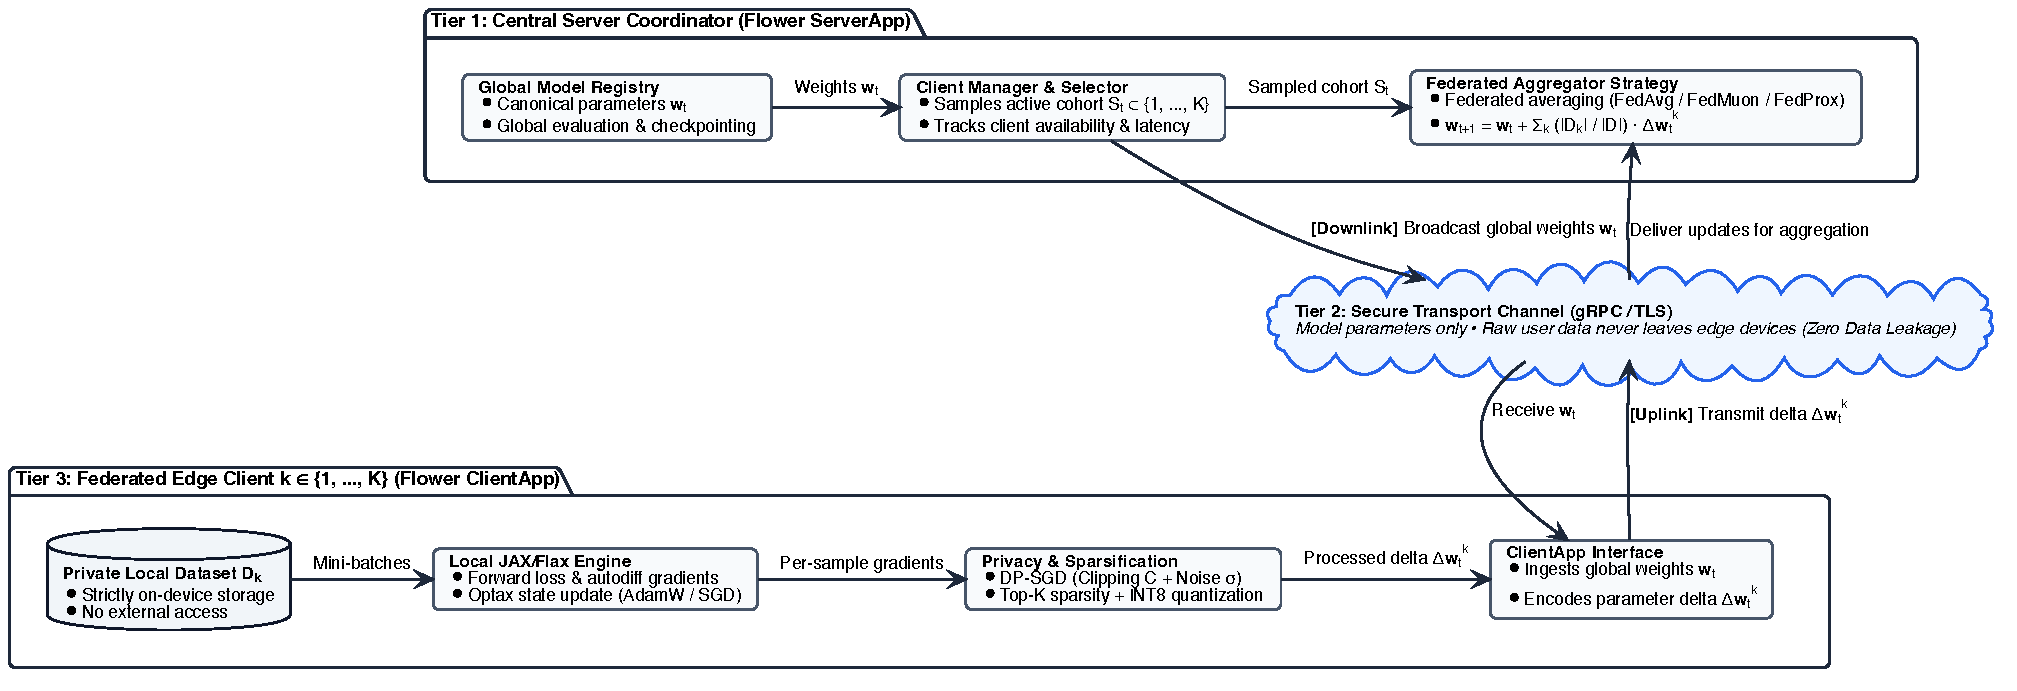
\includegraphics[width=\textwidth]{figures/fl_system_overview.pdf}
    \caption{Three-Tier Federated Learning Architecture (\texttt{fl\_system\_overview.svg}), illustrating the physical and logical decoupling of Central Orchestration, Secure Transport, and Distributed Edge Client execution.}
    \label{fig:fl_system_overview}
\end{figure}

\section{Executive Summary \& Elevator Pitch}
\begin{elevatorpitch}
\textbf{The Big Picture in 30 Seconds:}\\
Traditional centralized machine learning pulls everyone's private photos onto one central server. Federated learning flips this upside down: private data stays safely on user phones, and the model travels to the data!
\begin{itemize}[leftmargin=*,itemsep=2pt]
    \item \textbf{Tier 1 (The Coordinator)}: The central Flower server coordinates training rounds, samples available clients, and averages updates.
    \item \textbf{Tier 2 (The Secure Highway)}: An encrypted gRPC/TLS channel that carries model weights—never raw photos.
    \item \textbf{Tier 3 (The Edge Workers)}: Distributed edge devices running lightning-fast JAX/Flax for on-device training.
\end{itemize}
\textbf{Core Takeaway:} Zero raw data ever leaves the user's phone, giving an airtight privacy guarantee with maximum training efficiency.
\end{elevatorpitch}

\section{Component-by-Component Architectural Walkthrough}
\subsection{Tier 1: Central Server Coordinator (Flower \texttt{ServerApp})}
The central server acts as an orchestrator and aggregator. It does not train the model directly, nor does it hold training samples:
\begin{enumerate}[leftmargin=*]
    \item \textbf{Global Model Registry}: Maintains canonical model parameters $\mathbf{w}_t \in \mathbb{R}^D$. At each round $t$, it serializes $\mathbf{w}_t$ into portable arrays and evaluates the aggregated model on a centralized test set to track global loss and accuracy.
    \item \textbf{Client Manager \& Selector}: Manages the pool of registered edge devices $\{1, \dots, K\}$. In every round $t$, it samples an active cohort $S_t \subseteq \{1, \dots, K\}$ based on availability, battery health, and network connectivity.
    \item \textbf{Federated Aggregator Strategy}: Implements aggregation operators (e.g., FedAvg, FedProx, FedMuon). It takes client update deltas $\{\Delta\mathbf{w}_t^k\}_{k \in S_t}$ and executes a weighted reduction.
\end{enumerate}

\subsection{Tier 2: Secure Transport Channel (gRPC / TLS)}
The transport tier establishes mutual TLS (mTLS) encrypted streams between edge nodes and the central server. The network payload is strictly limited to model tensors and scalar metadata (number of local samples $|D_k|$ and training loss).

\subsection{Tier 3: Federated Edge Client (Flower \texttt{ClientApp})}
Each edge worker represents an autonomous client $k$:
\begin{enumerate}[leftmargin=*]
    \item \textbf{Private Local Dataset ($D_k$)}: Partitioned local data stored in secure on-device storage.
    \item \textbf{Local JAX/Flax Engine}: Compiles forward loss and autodiff functions via \texttt{jax.jit} and \texttt{jax.grad}. Model states are stepped using Optax optimizers (e.g., AdamW or SGD with momentum).
    \item \textbf{Privacy \& Compression Kernels}: Optional on-device defense engines. DP-SGD clips per-sample gradients to norm $C$ and adds Gaussian perturbation $\sigma$. Compression applies Top-$K$ sparsification and uniform INT8 quantization.
    \item \textbf{ClientApp Interface}: Computes the final parameter delta $\Delta\mathbf{w}_t^k = \mathbf{w}_{\text{local}} - \mathbf{w}_t$ and returns it to the server driver.
\end{enumerate}

\section{Theoretical Foundations \& Mathematical Formulations}
\begin{mathfoundation}
Federated learning optimizes a distributed empirical risk objective:
\begin{equation}
    \min_{\mathbf{w} \in \mathbb{R}^D} F(\mathbf{w}) \triangleq \sum_{k=1}^K p_k F_k(\mathbf{w}), \quad \text{where } p_k \triangleq \frac{|D_k|}{|D|}, \quad |D| = \sum_{k=1}^K |D_k|
\end{equation}
The local empirical risk for client $k$ is given by:
\begin{equation}
    F_k(\mathbf{w}) \triangleq \frac{1}{|D_k|} \sum_{\xi \in D_k} \ell(\mathbf{w}; \xi)
\end{equation}
In round $t$, the downlink broadcast transmits:
\begin{equation}
    \text{Downlink}(k) \gets \mathbf{w}_t, \quad \forall k \in S_t
\end{equation}
Each client performs $E$ local epochs starting from $\mathbf{w}_{t, 0}^k = \mathbf{w}_t$, producing local weights $\mathbf{w}_{t, E}^k$. The uplink payload is defined as:
\begin{equation}
    \Delta\mathbf{w}_t^k \triangleq \mathbf{w}_{t, E}^k - \mathbf{w}_t
\end{equation}
The server computes the aggregated update:
\begin{equation}
    \mathbf{w}_{t+1} = \mathbf{w}_t + \sum_{k \in S_t} \frac{|D_k|}{\sum_{j \in S_t} |D_j|} \Delta\mathbf{w}_t^k
\end{equation}
\end{mathfoundation}

\section{Architectural Justifications \& Design Choices}
\begin{itemize}[leftmargin=*]
    \item \textbf{Why JAX/Flax over PyTorch?} Pure functional transformations (\texttt{jax.jit}, \texttt{jax.vmap}) allow vectorized per-sample gradient computation without memory overhead, and PyTrees enable immutable weight manipulations that avoid in-place state corruption.
    \item \textbf{Why Transmit Parameter Deltas ($\Delta\mathbf{w}$) Instead of Absolute Weights?} Deltas centered around zero have lower dynamic range and higher sparsity, making them significantly more compressible via Top-$K$ and INT8 quantization.
\end{itemize}

\section{Advisor Defense Questions \& Model Answers}
\begin{defenseqa}{Client Availability \& System Stragglers}
\textbf{Question}: \textit{"What happens when a sampled client drops out or suffers extreme network latency during the round?"}\\
\textbf{Answer}: Flower ServerApp employs a synchronous timeout threshold with a minimum client quorum constraint $K_{\min} \le |S_t|$. If a client fails to return its \texttt{FitRes} payload before the deadline, the aggregator drops the straggler and re-normalizes the weights $p_k$ over the remaining responsive subset $S_t^{\text{valid}}$, preserving unbiased aggregation.
\end{defenseqa}

\begin{defenseqa}{Adversarial Client Model Poisoning}
\textbf{Question}: \textit{"Can a malicious edge client upload arbitrary weights to derail the global model?"}\\
\textbf{Answer}: Yes, under naive FedAvg. Our architecture supports robust aggregation strategies (FedMedian, FedTrimmedMean, and FedProx) which compute coordinate-wise medians or trim extreme update percentiles, providing resilience against Byzantine poisoning attacks up to a breakdown point of $50\%$.
\end{defenseqa}

% ==============================================================================
% CHAPTER 2: DATA FLOW & PREPROCESSING PIPELINE
% ==============================================================================
\chapter{End-to-End Data Ingestion \& Partitioning Pipeline}
\label{chap:data_pipeline}

\begin{figure}[htbp]
    \centering
    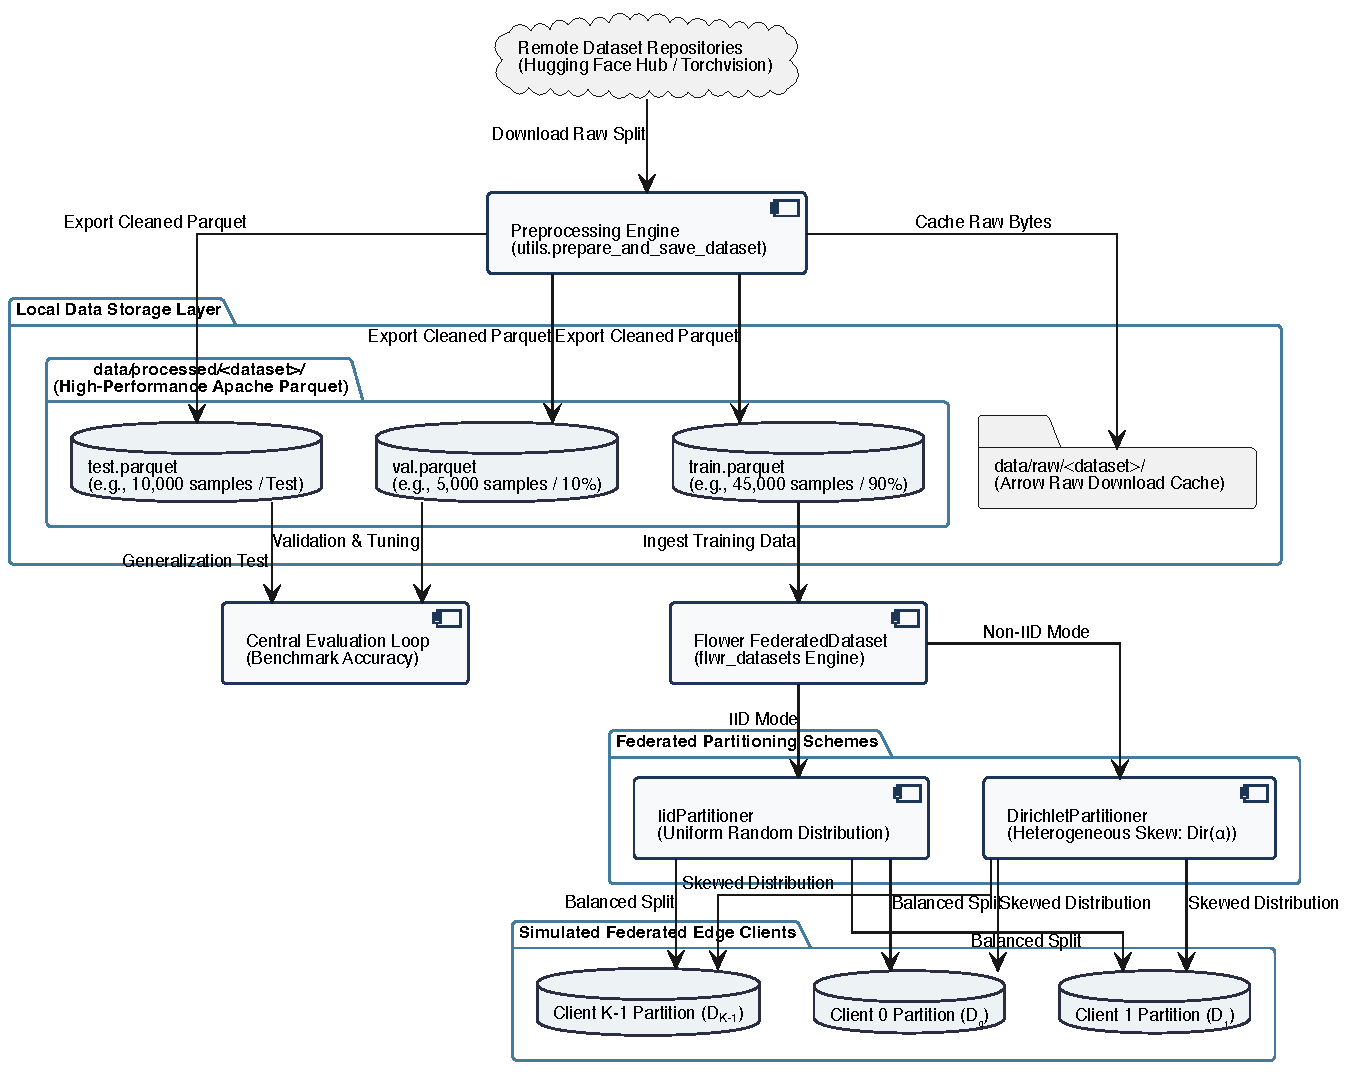
\includegraphics[width=\textwidth]{figures/data_flow_pipeline.pdf}
    \caption{Data Flow \& Preprocessing Pipeline (\texttt{data\_flow\_pipeline.svg}), tracing data transformation from remote repositories through columnar storage and non-IID partitioning to distributed client partitions.}
    \label{fig:data_flow_pipeline}
\end{figure}

\section{Executive Summary \& Elevator Pitch}
\begin{elevatorpitch}
Realistic federated benchmarks require rigorous simulation of non-identically distributed (non-IID) data across hundreds of clients. Our pipeline automates this process end-to-end:
\begin{enumerate}[leftmargin=*]
    \item Ingests raw splits from Hugging Face Hub or Torchvision.
    \item Converts raw samples into immutable, high-speed Apache Parquet files (\texttt{train}, \texttt{val}, \texttt{test}).
    \item Uses \texttt{flwr\_datasets} with Dirichlet ($\text{Dir}(\alpha)$) or Pathological partitioners to simulate heterogeneous statistical splits.
    \item Feeds clients balanced or skewed data while preserving an untouched test split for global benchmarking.
\end{enumerate}
\end{elevatorpitch}

\section{Component-by-Component Walkthrough}
\begin{itemize}[leftmargin=*]
    \item \textbf{Remote Repositories}: Raw datasets (e.g., CIFAR-10, MNIST, ImageNet) fetched over HTTPS.
    \item \textbf{Preprocessing Engine (\texttt{utils.prepare\_and\_save\_dataset})}: Validates schema, resizes image tensors, formats labels, and enforces a stratified validation split (e.g., $90\%$ train, $10\%$ val).
    \item \textbf{Storage Layer (\texttt{data/processed/\{dataset\}/})}: Apache Parquet format with columnar dictionary encoding and Snappy compression.
    \item \textbf{Flower FederatedDataset}: Bridges local Parquet tables with distributed partitioners.
    \item \textbf{Partitioning Schemes}:
        \begin{itemize}
            \item \textbf{IidPartitioner}: Uniform random permutation across client IDs.
            \item \textbf{DirichletPartitioner}: Parameterized by concentration $\alpha$, allocating class proportions according to a Dirichlet distribution.
        \end{itemize}
    \item \textbf{Simulated Edge Clients ($D_0, \dots, D_{K-1}$)}: Isolated client partitions consumed by local data loaders.
\end{itemize}

\section{Mathematical Modeling of Statistical Heterogeneity}
\begin{mathfoundation}
Let $C$ denote the number of classes and $K$ the number of edge clients. For each class $c \in \{1, \dots, C\}$, we sample a client proportion vector from a symmetric Dirichlet distribution:
\begin{equation}
    \mathbf{q}_c \sim \text{Dir}(\alpha \cdot \mathbf{1}_K), \quad \mathbf{q}_c = (q_{c, 1}, q_{c, 2}, \dots, q_{c, K}), \quad \sum_{k=1}^K q_{c, k} = 1
\end{equation}
where $\alpha > 0$ is the concentration parameter:
\begin{itemize}
    \item As $\alpha \to \infty$, $q_{c, k} \to 1/K$, recovering an identical (IID) distribution.
    \item As $\alpha \to 0^+$, $\mathbf{q}_c$ collapses into a one-hot vector, yielding extreme pathological skew where each client possesses only a single class.
\end{itemize}
Client $k$'s empirical label distribution $P_k(Y)$ is given by:
\begin{equation}
    P_k(Y = c) = \frac{q_{c, k} \cdot N_c}{\sum_{j=1}^C q_{j, k} \cdot N_j}
\end{equation}
The statistical discrepancy between client $k$ and client $j$ is quantified by Total Variation (TV) distance:
\begin{equation}
    D_{\text{TV}}(P_k, P_j) \triangleq \frac{1}{2} \sum_{c=1}^C |P_k(Y = c) - P_j(Y = c)| \in [0, 1]
\end{equation}
\end{mathfoundation}

\section{Advisor Defense Questions \& Model Answers}
\begin{defenseqa}{Dirichlet Concentration Parameter $\alpha$}
\textbf{Question}: \textit{"Why did you benchmark using $\alpha = 0.1$ and $\alpha = 0.5$ instead of just IID data?"}\\
\textbf{Answer}: Real-world mobile and edge datasets exhibit extreme label skew. Under standard IID assumptions, simple FedAvg converges rapidly. However, at $\alpha = 0.1$, client drift $\|\mathbf{w}_t^k - \mathbf{w}_t\|$ escalates dramatically because local gradients point toward incompatible loss minima. Benchmarking under low $\alpha$ is essential to demonstrate the superiority of robust aggregation methods like FedProx and FedMuon.
\end{defenseqa}

% ==============================================================================
% CHAPTER 3: JAX/FLAX NEURAL MODEL ARCHITECTURES
% ==============================================================================
\chapter{JAX/Flax Neural Model Architecture Hierarchy}
\label{chap:models}

\begin{figure}[htbp]
    \centering
    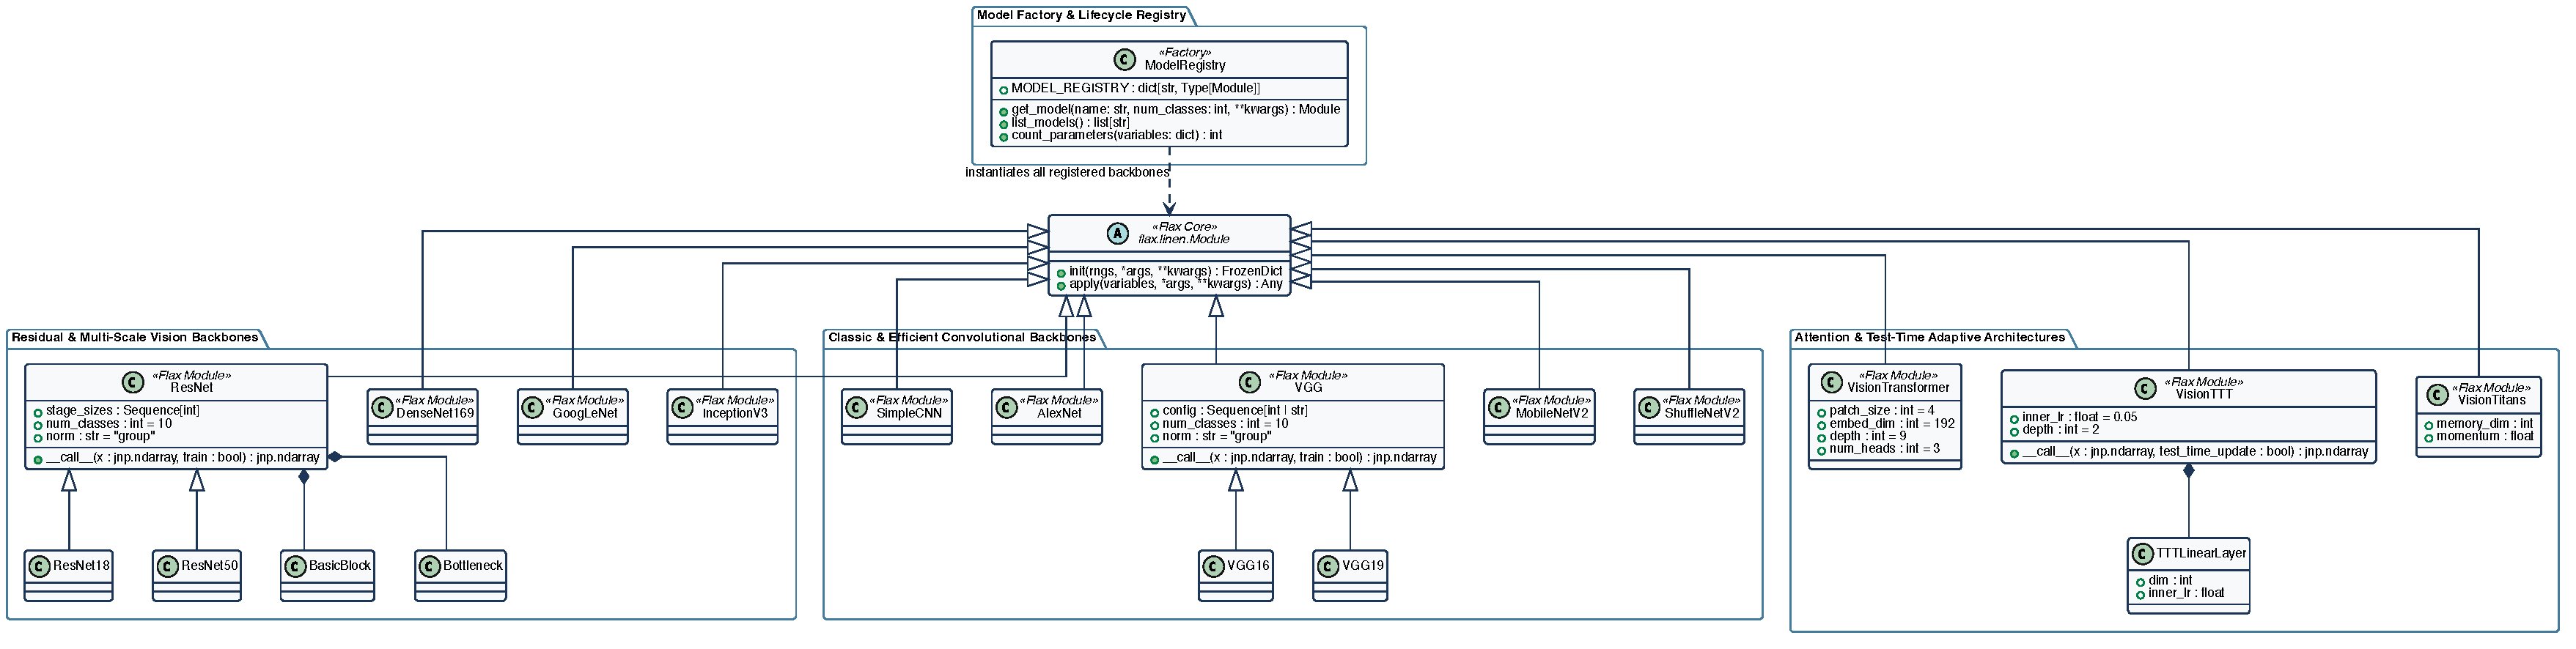
\includegraphics[width=\textwidth]{figures/model_architectures.pdf}
    \caption{Flax Linen Neural Model Backbone Hierarchy (\texttt{model\_architectures.svg}), demonstrating the object-oriented structure and module inheritance across CNNs, Transformers, and Test-Time Training backbones.}
    \label{fig:model_architectures}
\end{figure}

\section{Executive Summary \& Elevator Pitch}
\begin{elevatorpitch}
Federated learning across diverse edge hardware requires modular, swappable backbones. Our model repository is built on \texttt{flax.linen.Module}, encompassing:
\begin{itemize}[leftmargin=*]
    \item \textbf{Residual \& Multi-Scale}: ResNet (18/34/50), DenseNet-169, GoogLeNet, InceptionV3.
    \item \textbf{Efficient Edge CNNs}: MobileNetV2, ShuffleNetV2, VGG (16/19), SimpleCNN.
    \item \textbf{Adaptive Foundations}: Vision Transformer (ViT), Test-Time Training (VisionTTT), and Titans Neural Long-Term Memory.
\end{itemize}
All models conform to a unified factory interface managed by \texttt{ModelRegistry}.
\end{elevatorpitch}

\section{Component-by-Component Walkthrough}
\begin{itemize}[leftmargin=*]
    \item \textbf{\texttt{flax.linen.Module}}: Pure functional base class. Decouples state manipulation from computation through \texttt{init(rng, x)} and \texttt{apply(params, x)}.
    \item \textbf{\texttt{ResNet} with BasicBlock \& Bottleneck}: Residual networks employing shortcut connections $\mathbf{y} = \mathcal{F}(\mathbf{x}) + \mathbf{x}$. Group Normalization is utilized in place of Batch Normalization to prevent non-IID statistical collapse.
    \item \textbf{\texttt{VisionTransformer} (ViT)}: Computes patch embeddings via non-overlapping 2D convolutions, followed by Multi-Head Self-Attention (MHSA) and MLP feed-forward blocks.
    \item \textbf{\texttt{VisionTTT} (Test-Time Training)}: Features an inner-loop self-supervised gradient update on test samples before making downstream predictions.
    \item \textbf{\texttt{ModelRegistry}}: Central factory providing reflection, instantiation, parameter accounting, and metadata inspection.
\end{itemize}

\section{Mathematical Formulations of Modern Backbones}
\begin{mathfoundation}
\textbf{1. Residual Learning Formulation}:
\begin{equation}
    \mathbf{x}_{l+1} = \mathbf{x}_l + \mathcal{F}(\mathbf{x}_l, \mathcal{W}_l), \quad \text{ensuring } \frac{\partial \mathcal{E}}{\partial \mathbf{x}_l} = \frac{\partial \mathcal{E}}{\partial \mathbf{x}_L} \left( \mathbf{I} + \frac{\partial}{\partial \mathbf{x}_l} \sum_{i=l}^{L-1} \mathcal{F}_i \right)
\end{equation}
which preserves non-vanishing gradient flow across deep networks.

\textbf{2. Vision Transformer Attention}:
For patch sequence $\mathbf{Z} \in \mathbb{R}^{N \times D}$, query, key, and value projections $\mathbf{Q}, \mathbf{K}, \mathbf{V}$ yield:
\begin{equation}
    \text{Attention}(\mathbf{Q}, \mathbf{K}, \mathbf{V}) = \text{softmax}\left( \frac{\mathbf{Q} \mathbf{K}^T}{\sqrt{d_k}} \right) \mathbf{V}
\end{equation}

\textbf{3. Test-Time Training (TTT) Adaptation}:
At test time, the feature representation is updated on incoming batch $\mathbf{x}_{\text{test}}$ via self-supervised task loss $\mathcal{L}_{\text{self}}$:
\begin{equation}
    \bm{\theta}^*_{\text{test}} = \bm{\theta} - \eta_{\text{inner}} \nabla_{\bm{\theta}} \mathcal{L}_{\text{self}}(\bm{\theta}; \mathbf{x}_{\text{test}})
\end{equation}
before computing classification logits $\hat{\mathbf{y}} = g(\mathbf{x}_{\text{test}}; \bm{\theta}^*_{\text{test}})$.
\end{mathfoundation}

\section{Advisor Defense Questions \& Model Answers}
\begin{defenseqa}{Group Normalization vs. Batch Normalization in FL}
\textbf{Question}: \textit{"Why did you substitute Group Normalization for standard Batch Normalization across all convolutional models?"}\\
\textbf{Answer}: In Batch Normalization, running mean $\mu_B$ and variance $\sigma_B^2$ depend on local batch statistics. Under non-IID client data, local batch statistics diverge drastically between clients. Aggregating these disparate running statistics during server averaging leads to severe internal covariate shift and catastrophic test accuracy degradation. Group Normalization computes statistics along feature channels for each sample independently:
\begin{equation}
    \mu_{n, g} = \frac{1}{(C/G)HW} \sum_{c \in S_g} \sum_{h, w} x_{n, c, h, w}
\end{equation}
rendering normalization completely invariant to batch size and client label distribution.
\end{defenseqa}

% ==============================================================================
% CHAPTER 4: DATA ENGINEERING & PARTITIONING CLASS HIERARCHY
% ==============================================================================
\chapter{Data Engineering \& Partitioning Class Hierarchy}
\label{chap:data_classes}

\begin{figure}[htbp]
    \centering
    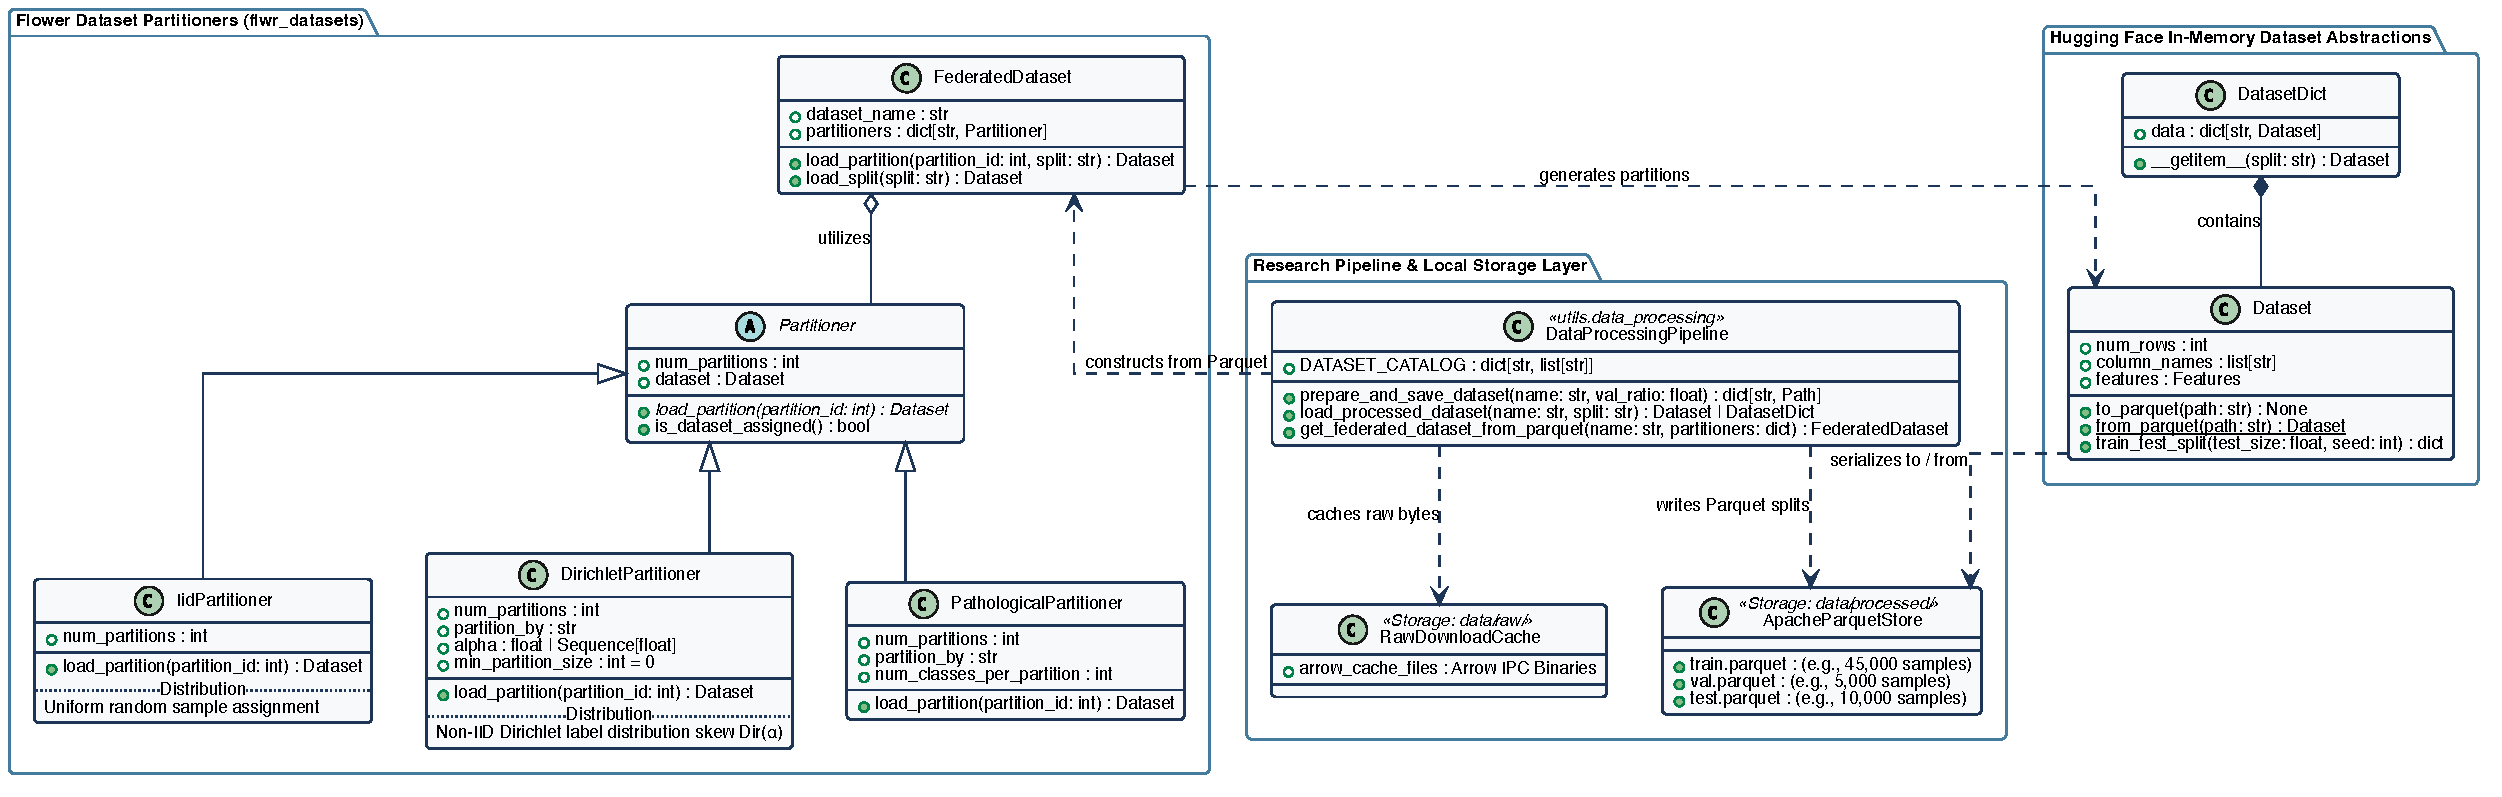
\includegraphics[width=\textwidth]{figures/data_pipeline_classes.pdf}
    \caption{Data Engineering Class Diagram (\texttt{data\_pipeline\_classes.svg}), depicting partitioner abstractions, in-memory dataset contracts, and high-performance Parquet storage pipelines.}
    \label{fig:data_pipeline_classes}
\end{figure}

\section{Executive Summary \& Elevator Pitch}
\begin{elevatorpitch}
To guarantee experimental reproducibility and high-throughput execution during federated simulation, the data layer decouples raw disk ingestion from in-memory partition sampling. The class hierarchy provides:
\begin{itemize}[leftmargin=*]
    \item Abstract \texttt{Partitioner} base classes with concrete Dirichlet, IID, and Pathological partitioners.
    \item High-speed zero-copy access via Hugging Face \texttt{Dataset} and \texttt{DatasetDict}.
    \item Columnar persistence in Apache Parquet format.
\end{itemize}
\end{elevatorpitch}

\section{Class-by-Class Breakdown}
\begin{itemize}[leftmargin=*]
    \item \textbf{\texttt{Partitioner} (Abstract Base Class)}: Defines the interface \texttt{load\_partition(partition\_id: int) -> Dataset}.
    \item \textbf{\texttt{IidPartitioner}}: Assigns sample indices uniformly across partitions via pseudorandom shuffle.
    \item \textbf{\texttt{DirichletPartitioner}}: Accepts concentration parameter $\alpha$ and optional \texttt{min\_partition\_size} to prevent empty client allocations.
    \item \textbf{\texttt{PathologicalPartitioner}}: Assigns exactly $S$ unique classes to each client, simulating domain specialization.
    \item \textbf{\texttt{FederatedDataset}}: Composite wrapper providing unified access across multiple splits.
    \item \textbf{\texttt{DataProcessingPipeline}}: Manages automated caching, validation splits, and Parquet export.
\end{itemize}

\section{Advisor Defense Questions \& Model Answers}
\begin{defenseqa}{Zero-Copy Memory-Mapped Access}
\textbf{Question}: \textit{"Why did you adopt Apache Parquet over traditional PyTorch ImageFolder or raw SQLite databases?"}\\
\textbf{Answer}: Parquet uses columnar encoding with Snappy compression, reducing disk footprint by $60\text{--}80\%$ compared to raw image folders. Combined with Apache Arrow, datasets can be memory-mapped directly from disk without serializing Python objects, eliminating memory duplication during large-scale federated simulations with 100+ simulated edge clients.
\end{defenseqa}

% ==============================================================================
% CHAPTER 5: FEDERATED TRAINING ROUND LIFECYCLE
% ==============================================================================
\chapter{Federated Training Round Sequence Lifecycle}
\label{chap:round_lifecycle}

\begin{figure}[htbp]
    \centering
    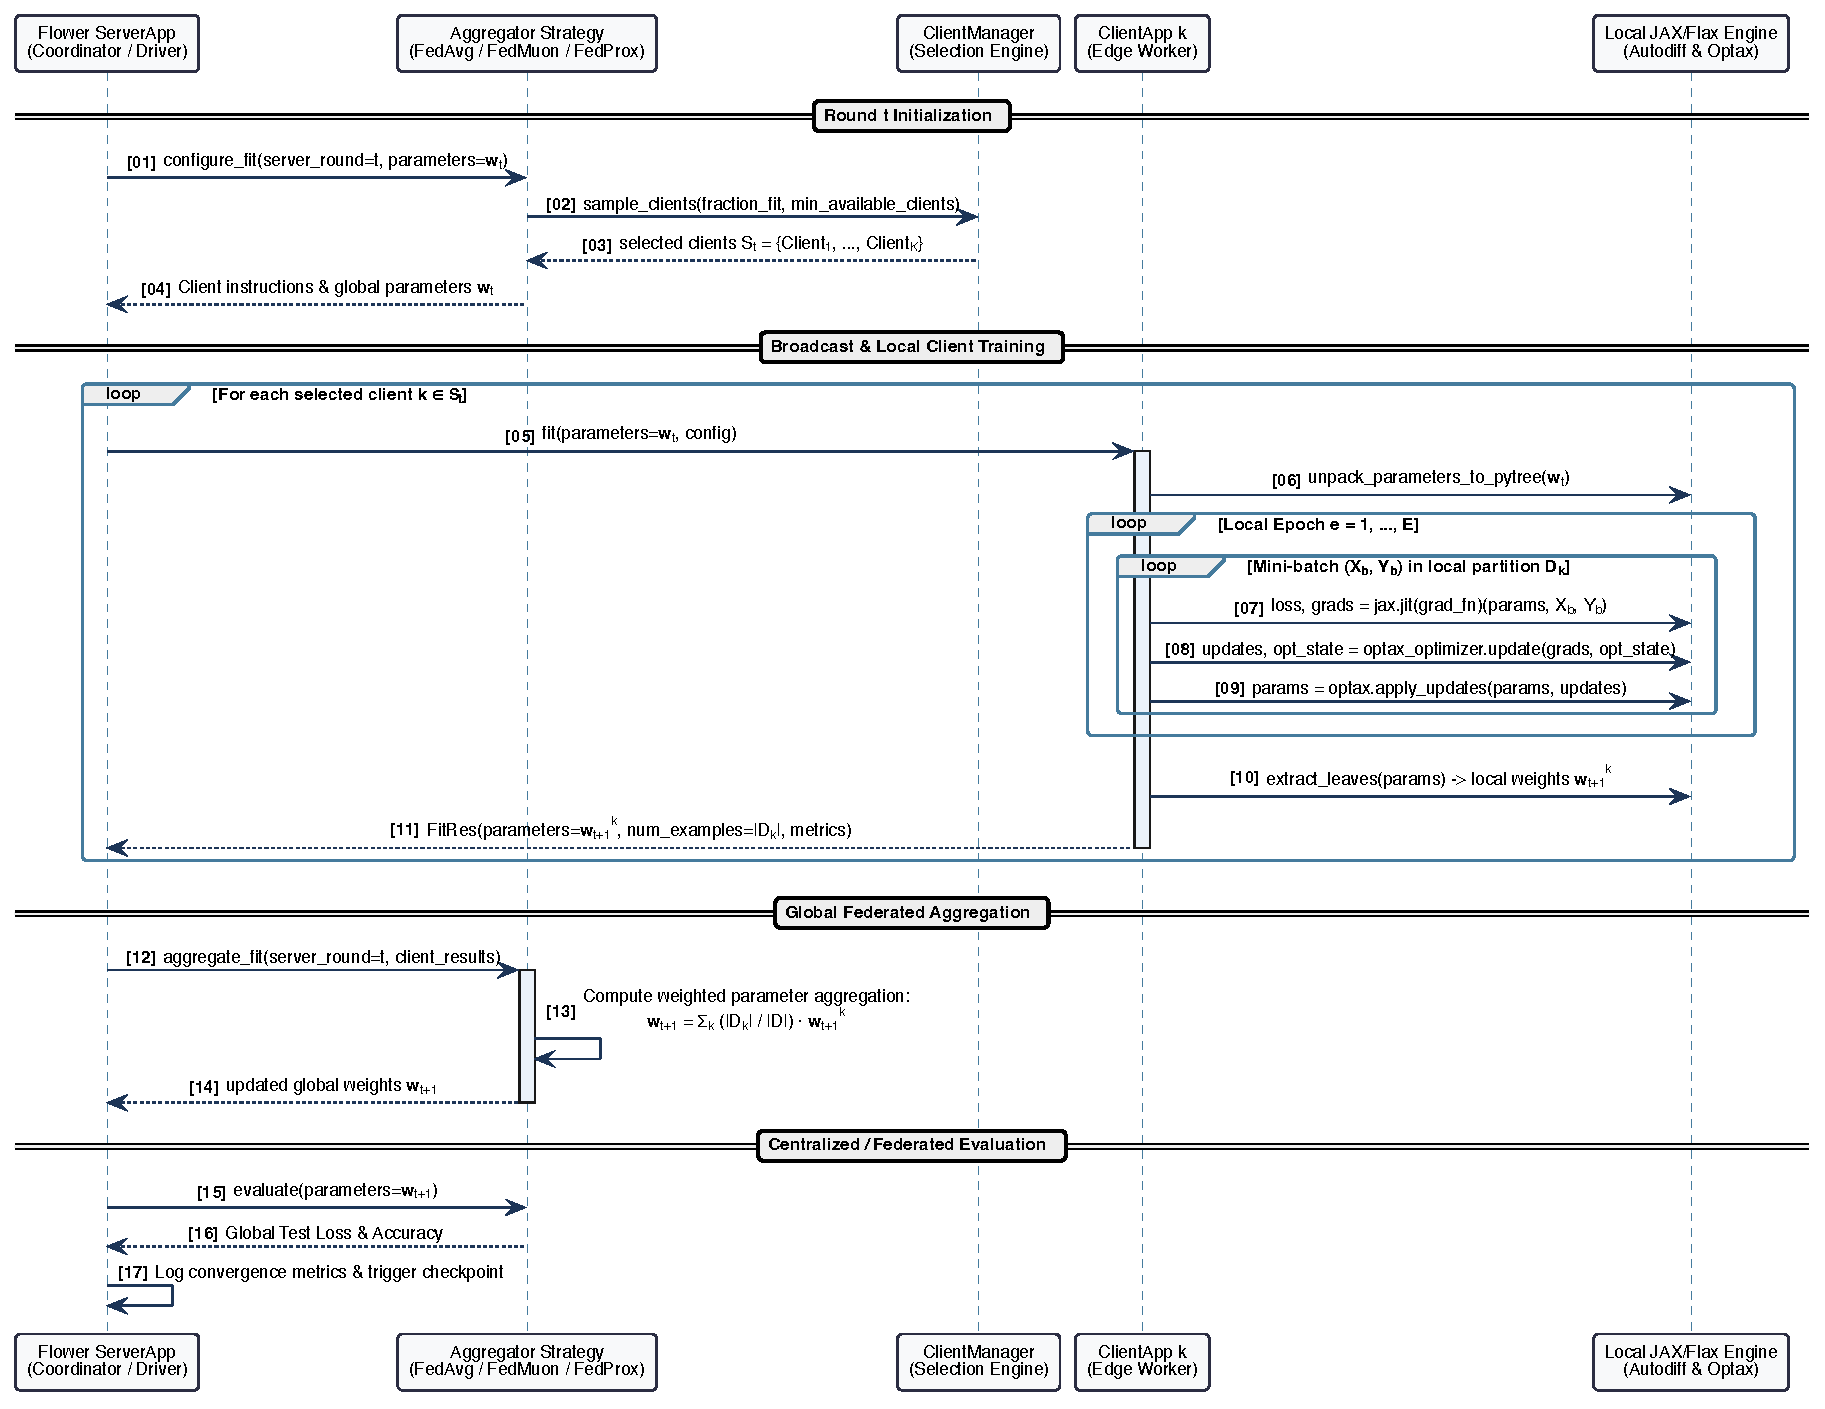
\includegraphics[width=\textwidth]{figures/fl_training_round.pdf}
    \caption{Federated Training Round Sequence (\texttt{fl\_training\_round.svg}), illustrating the step-by-step synchronous message-passing lifecycle between ServerApp, Strategy, ClientManager, and ClientApp.}
    \label{fig:fl_training_round}
\end{figure}

\section{Executive Summary \& Elevator Pitch}
\begin{elevatorpitch}
A federated training round is a distributed synchronous protocol:
\begin{enumerate}[leftmargin=*]
    \item The server queries the Strategy to configure the round and sample clients via the \texttt{ClientManager}.
    \item Global parameters $\mathbf{w}_t$ are broadcast to the selected cohort $S_t$.
    \item Each client executes local training on private mini-batches using JIT-compiled JAX kernels.
    \item Clients return updated parameters $\mathbf{w}_{t+1}^k$ and sample counts $|D_k|$.
    \item The strategy computes a weighted reduction, evaluates global performance, and records metrics.
\end{enumerate}
\end{elevatorpitch}

\section{Sequence Step-by-Step Breakdown}
\begin{itemize}[leftmargin=*]
    \item \textbf{Step [01--04] Round Initialization}: \texttt{ServerApp} invokes \texttt{Strategy.configure\_fit}. The strategy instructs \texttt{ClientManager} to sample active cohort $S_t$.
    \item \textbf{Step [05--06] Broadcast}: Server dispatches \texttt{fit()} RPC instructions carrying global weights $\mathbf{w}_t$ to each client $k \in S_t$.
    \item \textbf{Step [07--11] Local JAX Execution}: Client unpacks weights into a Flax PyTree and executes $E$ local epochs over mini-batches $(X_b, Y_b)$, applying Optax optimizer updates.
    \item \textbf{Step [12--13] Uplink Response}: Client packages trained weights $\mathbf{w}_{t+1}^k$ and sample count $|D_k|$ into a \texttt{FitRes} response.
    \item \textbf{Step [14--16] Aggregation \& Evaluation}: Strategy executes weighted aggregation, evaluates the new model $\mathbf{w}_{t+1}$ on the centralized validation set, and saves a checkpoint.
\end{itemize}

\section{Mathematical Formulation of Federated Aggregation Strategies}
\begin{mathfoundation}
\textbf{1. Standard FedAvg (McMahan et al.)}:
\begin{equation}
    \mathbf{w}_{t+1} = \sum_{k \in S_t} \frac{|D_k|}{\sum_{j \in S_t} |D_j|} \mathbf{w}_{t+1}^k
\end{equation}

\textbf{2. FedProx (Li et al.)}:
Adds a proximal regularization term to each client's local loss to penalize divergence from the global model:
\begin{equation}
    \min_{\mathbf{w}} h_k(\mathbf{w}; \mathbf{w}_t) \triangleq F_k(\mathbf{w}) + \frac{\mu}{2} \|\mathbf{w} - \mathbf{w}_t\|_2^2
\end{equation}
where $\mu \ge 0$ stabilizes optimization under severe statistical heterogeneity ($\alpha < 0.5$).

\textbf{3. FedMuon (Momentum Orthogonalized Aggregator)}:
Applies a matrix-momentum update orthogonalized via Newton-Schulz iterations:
\begin{equation}
    \mathbf{G}_{t} = \sum_{k \in S_t} p_k \Delta\mathbf{w}_t^k, \quad \mathbf{M}_t = \beta \mathbf{M}_{t-1} + (1 - \beta) \mathbf{G}_t
\end{equation}
followed by approximate polar decomposition $\mathbf{O}_t \approx \text{Polar}(\mathbf{M}_t)$ to maintain uniform update energy across all parameter layers.
\end{mathfoundation}

\section{Advisor Defense Questions \& Model Answers}
\begin{defenseqa}{Client Drift in Non-IID Regimes}
\textbf{Question}: \textit{"Why does standard FedAvg exhibit objective inconsistency when client data is non-IID?"}\\
\textbf{Answer}: When local datasets $D_k$ are heterogeneous, local loss minima $\mathbf{w}_k^* = \arg\min F_k(\mathbf{w})$ do not align with the global minimum $\mathbf{w}^* = \arg\min F(\mathbf{w})$. During multiple local epochs ($E > 1$), local gradient steps pull each client toward its local minimum $\mathbf{w}_k^*$. Averaging these drifted weights causes the trajectory to diverge from the true global optimum:
\begin{equation}
    \|\mathbf{w}_{t+1} - \mathbf{w}^*\| \le \rho \|\mathbf{w}_t - \mathbf{w}^*\| + \mathcal{O}\left( \eta \sum_{k=1}^K p_k \|\nabla F_k(\mathbf{w}^*) - \nabla F(\mathbf{w}^*)\| \right)
\end{equation}
FedProx bounds this drift by enforcing the proximal penalty $\frac{\mu}{2}\|\mathbf{w} - \mathbf{w}_t\|^2$, guaranteeing stable convergence.
\end{defenseqa}

% ==============================================================================
% CHAPTER 6: DIFFERENTIAL PRIVACY VIA DP-SGD
% ==============================================================================
\chapter{Differential Privacy via DP-SGD}
\label{chap:dp_sgd}

\begin{figure}[htbp]
    \centering
    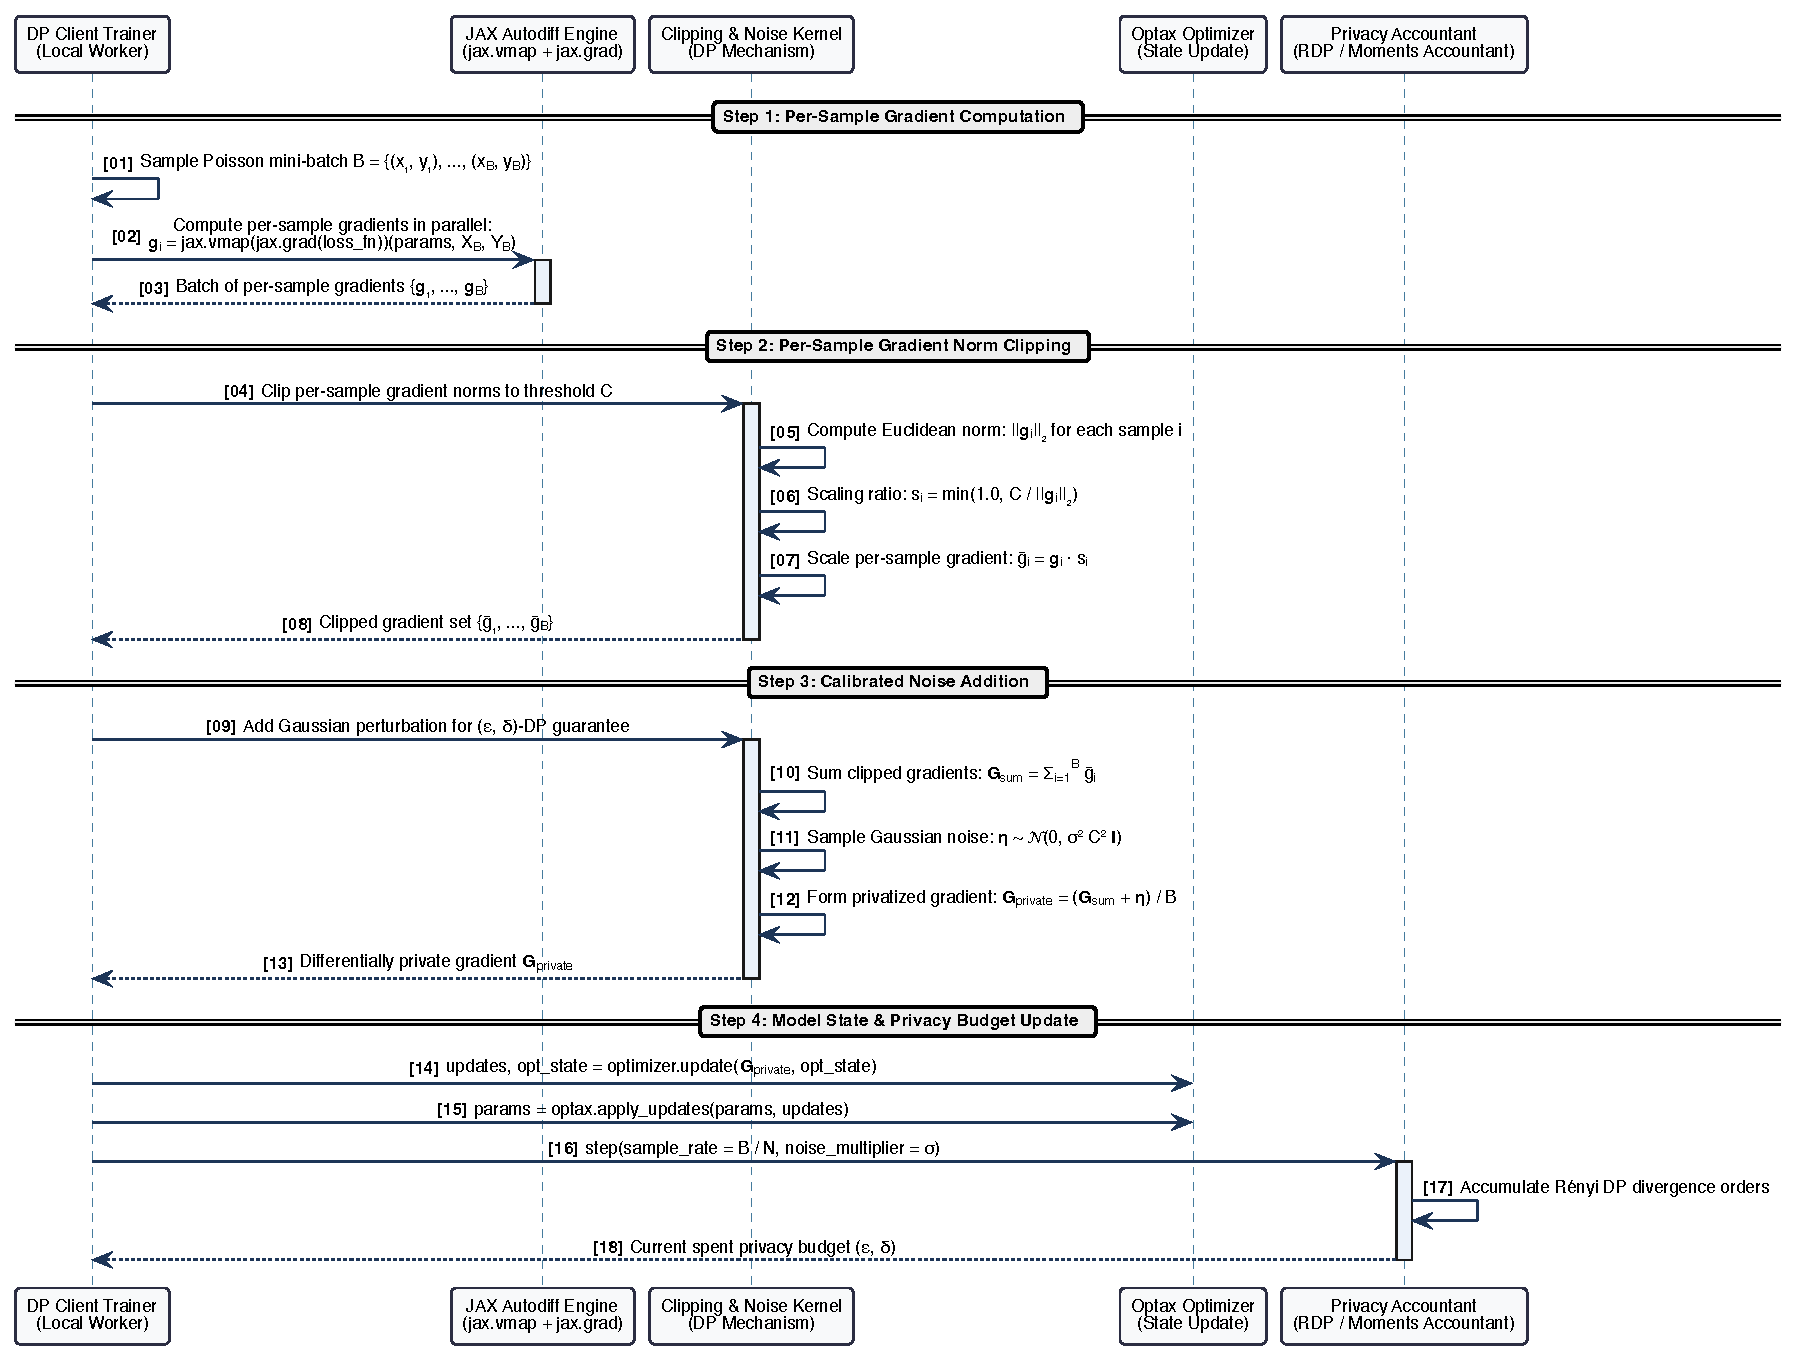
\includegraphics[width=\textwidth]{figures/differential_privacy_dp_sgd.pdf}
    \caption{Differentially Private SGD Sequence (\texttt{differential\_privacy\_dp\_sgd.svg}), demonstrating per-sample gradient computation, $L_2$ norm clipping, Gaussian perturbation, and Rényi privacy accounting.}
    \label{fig:differential_privacy_dp_sgd}
\end{figure}

\section{Executive Summary \& Elevator Pitch}
\begin{elevatorpitch}
Although federated learning prevents raw data transmission, deep neural networks remain vulnerable to gradient inversion attacks (e.g., DLG, Inverting Gradients) which can reconstruct training images from parameter updates. We mitigate this through on-device Differentially Private SGD (DP-SGD):
\begin{enumerate}[leftmargin=*]
    \item Computes exact per-sample gradients in parallel via \texttt{jax.vmap}.
    \item Clips per-sample gradient $L_2$ norms to threshold $C$.
    \item Injects calibrated Gaussian noise $\mathcal{N}(0, \sigma^2 C^2 \mathbf{I})$.
    \item Tracks privacy expenditure $(\epsilon, \delta)$ using a Rényi Differential Privacy (RDP) accountant.
\end{enumerate}
\end{elevatorpitch}

\section{Sequence Step-by-Step Breakdown}
\begin{itemize}[leftmargin=*]
    \item \textbf{Step 1: Per-Sample Gradient Computation}: Generates mini-batch $B$ via Poisson subsampling and evaluates $\mathbf{g}_i = \nabla_{\mathbf{w}} \ell(\mathbf{w}; x_i, y_i)$ for each sample $i$ independently.
    \item \textbf{Step 2: Gradient Norm Clipping}: Clips each per-sample gradient to norm threshold $C$:
    \begin{equation}
        \bar{\mathbf{g}}_i = \mathbf{g}_i \cdot \min\left(1, \frac{C}{\|\mathbf{g}_i\|_2}\right)
    \end{equation}
    ensuring global $L_2$ sensitivity is strictly bounded by $C$.
    \item \textbf{Step 3: Calibrated Noise Addition}: Aggregates clipped gradients and injects isotropic Gaussian noise:
    \begin{equation}
        \tilde{\mathbf{g}} = \frac{1}{|B|} \left( \sum_{i=1}^{|B|} \bar{\mathbf{g}}_i + \mathcal{N}\left(0, \sigma^2 C^2 \mathbf{I}\right) \right)
    \end{equation}
    \item \textbf{Step 4: Optax State \& Budget Tracking}: Applies privatized gradient $\tilde{\mathbf{g}}$ to local model weights and advances the RDP privacy accountant.
\end{itemize}

\section{Theoretical Foundations \& Privacy Guarantees}
\begin{mathfoundation}
A randomized algorithm $\mathcal{M}$ satisfies $(\epsilon, \delta)$-Differential Privacy if for any two adjacent datasets $D, D'$ differing by at most one sample ($|D \Delta D'| = 1$), and for any set of outputs $\mathcal{S} \subseteq \text{Range}(\mathcal{M})$:
\begin{equation}
    \mathbb{P}[\mathcal{M}(D) \in \mathcal{S}] \le e^\epsilon \cdot \mathbb{P}[\mathcal{M}(D') \in \mathcal{S}] + \delta
\end{equation}
Under Gaussian perturbation with subsampling ratio $q = |B|/|D_k|$ and noise multiplier $\sigma$, the Rényi Differential Privacy (RDP) of order $\alpha > 1$ accumulates linearly across $T$ iterations:
\begin{equation}
    \epsilon_{\text{total}}(\alpha) = T \cdot \epsilon_{\mathcal{M}}(\alpha)
\end{equation}
Converting from RDP to standard $(\epsilon, \delta)$-DP yields:
\begin{equation}
    \epsilon(\delta) = \min_{\alpha > 1} \left( \epsilon_{\text{total}}(\alpha) + \frac{\log(1/\delta)}{\alpha - 1} \right) = \mathcal{O}\left( \frac{q \sqrt{T \log(1/\delta)}}{\sigma} \right)
\end{equation}
\end{mathfoundation}

\section{Advisor Defense Questions \& Model Answers}
\begin{defenseqa}{Clipping Bias vs. Noise Variance}
\textbf{Question}: \textit{"How does gradient clipping affect model convergence, and how is the clipping threshold $C$ calibrated?"}\\
\textbf{Answer}: Clipping introduces directional bias by truncating outlier gradients:
\begin{equation}
    \mathbb{E}[\bar{\mathbf{g}}] = \mathbb{E}\left[ \mathbf{g} \cdot \min\left(1, \frac{C}{\|\mathbf{g}\|_2}\right) \right] \ne \mathbb{E}[\mathbf{g}]
\end{equation}
If $C$ is too small, gradient signals are over-clipped, slowing convergence. If $C$ is too large, the required noise scale $\sigma^2 C^2 \mathbf{I}$ drowns out the gradient signal. We calibrate $C$ to match the median gradient norm across initial epochs ($C \approx \text{median}(\|\mathbf{g}_i\|_2)$), maintaining balance between bias and noise variance.
\end{defenseqa}

% ==============================================================================
% CHAPTER 7: EDGE CLIENT LOCAL EXECUTION LIFECYCLE
% ==============================================================================
\chapter{Edge Client Local Execution Lifecycle}
\label{chap:client_lifecycle}

\begin{figure}[htbp]
    \centering
    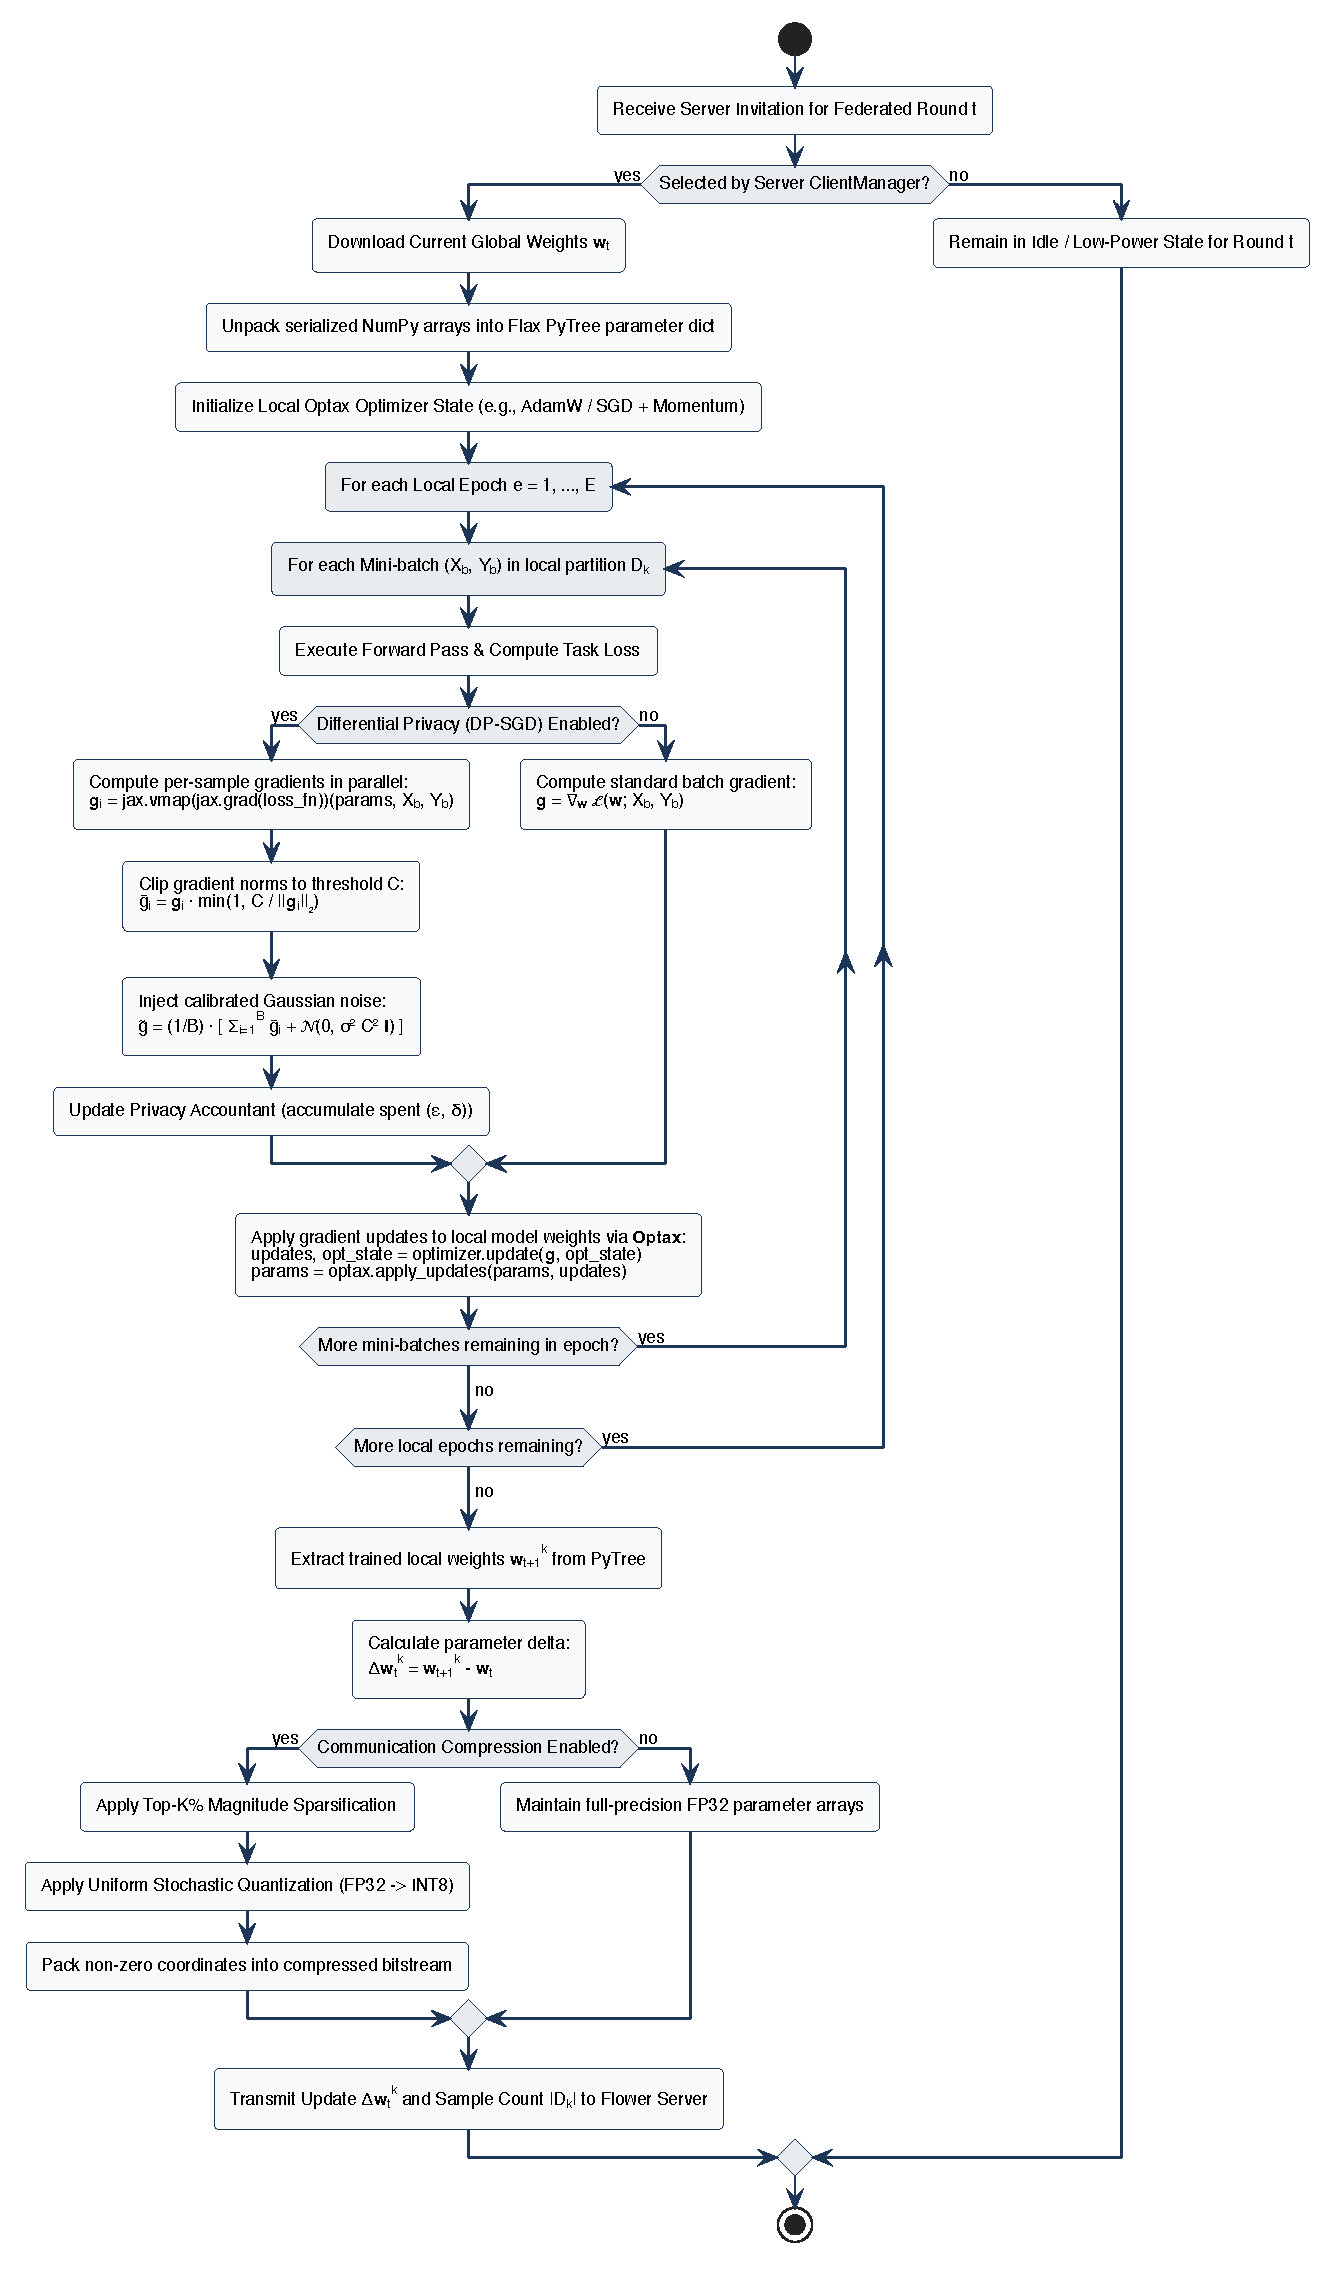
\includegraphics[width=0.85\textwidth,height=0.65\textheight,keepaspectratio]{figures/client_execution_lifecycle.pdf}
    \caption{Edge Client Execution Lifecycle (\texttt{client\_execution\_lifecycle.svg}), illustrating the on-device execution state machine across sampling, training, privacy, compression, and uplink transmission.}
    \label{fig:client_execution_lifecycle}
\end{figure}

\section{Executive Summary \& Elevator Pitch}
\begin{elevatorpitch}
Edge devices operate under strict compute, memory, and battery constraints. The client execution lifecycle is a deterministic state machine:
\begin{itemize}[leftmargin=*]
    \item Responds to server invitations and enters low-power idle mode when not selected.
    \item Unpacks weights into local Flax PyTrees and initializes Optax states.
    \item Runs localized training loops with configurable DP-SGD branches.
    \item Produces parameter deltas $\Delta\mathbf{w}_t^k$ with optional Top-$K$ and INT8 compression before uplink transmission.
\end{itemize}
\end{elevatorpitch}

\section{Activity Flowchart Breakdown}
\begin{itemize}[leftmargin=*]
    \item \textbf{Selection Guard}: Verifies whether client ID belongs to active cohort $S_t$. If not selected, the client remains idle to conserve battery and compute.
    \item \textbf{State Ingestion}: Ingests serialized NumPy buffers, reconstructs the Flax PyTree parameter dictionary, and initializes Optax optimizer momentum buffers.
    \item \textbf{Nested Epoch \& Batch Loops}: Iterates across $E$ epochs and mini-batches $(X_b, Y_b)$, executing forward loss computation, autodiff, and weight updates.
    \item \textbf{Privacy Conditional}: Evaluates whether DP-SGD is enabled. If active, runs vectorized per-sample clipping and noise injection; otherwise, computes standard batch gradients.
    \item \textbf{Delta Calculation}: Computes parameter delta $\Delta\mathbf{w}_t^k = \mathbf{w}_{t+1}^k - \mathbf{w}_t$.
    \item \textbf{Compression Conditional}: If active, applies Top-$K$ magnitude thresholding and uniform INT8 quantization before transmission.
\end{itemize}

\section{Advisor Defense Questions \& Model Answers}
\begin{defenseqa}{Local Epoch Trade-off ($E$)}
\textbf{Question}: \textit{"What is the trade-off in setting local epochs $E = 1$ versus $E = 10$?"}\\
\textbf{Answer}: Increasing local epochs $E$ allows clients to perform more computation per communication round, reducing total communication overhead. However, when local data is non-IID, larger $E$ accelerates client drift, causing local models to overfit to their local data distributions and degrading global model convergence. Tuning $E \in [1, 5]$ balances communication savings against client drift.
\end{defenseqa}

% ==============================================================================
% CHAPTER 8: COMMUNICATION EFFICIENCY & COMPRESSION PIPELINE
% ==============================================================================
\chapter{Communication Efficiency \& Gradient Compression}
\label{chap:comm_efficiency}

\begin{figure}[htbp]
    \centering
    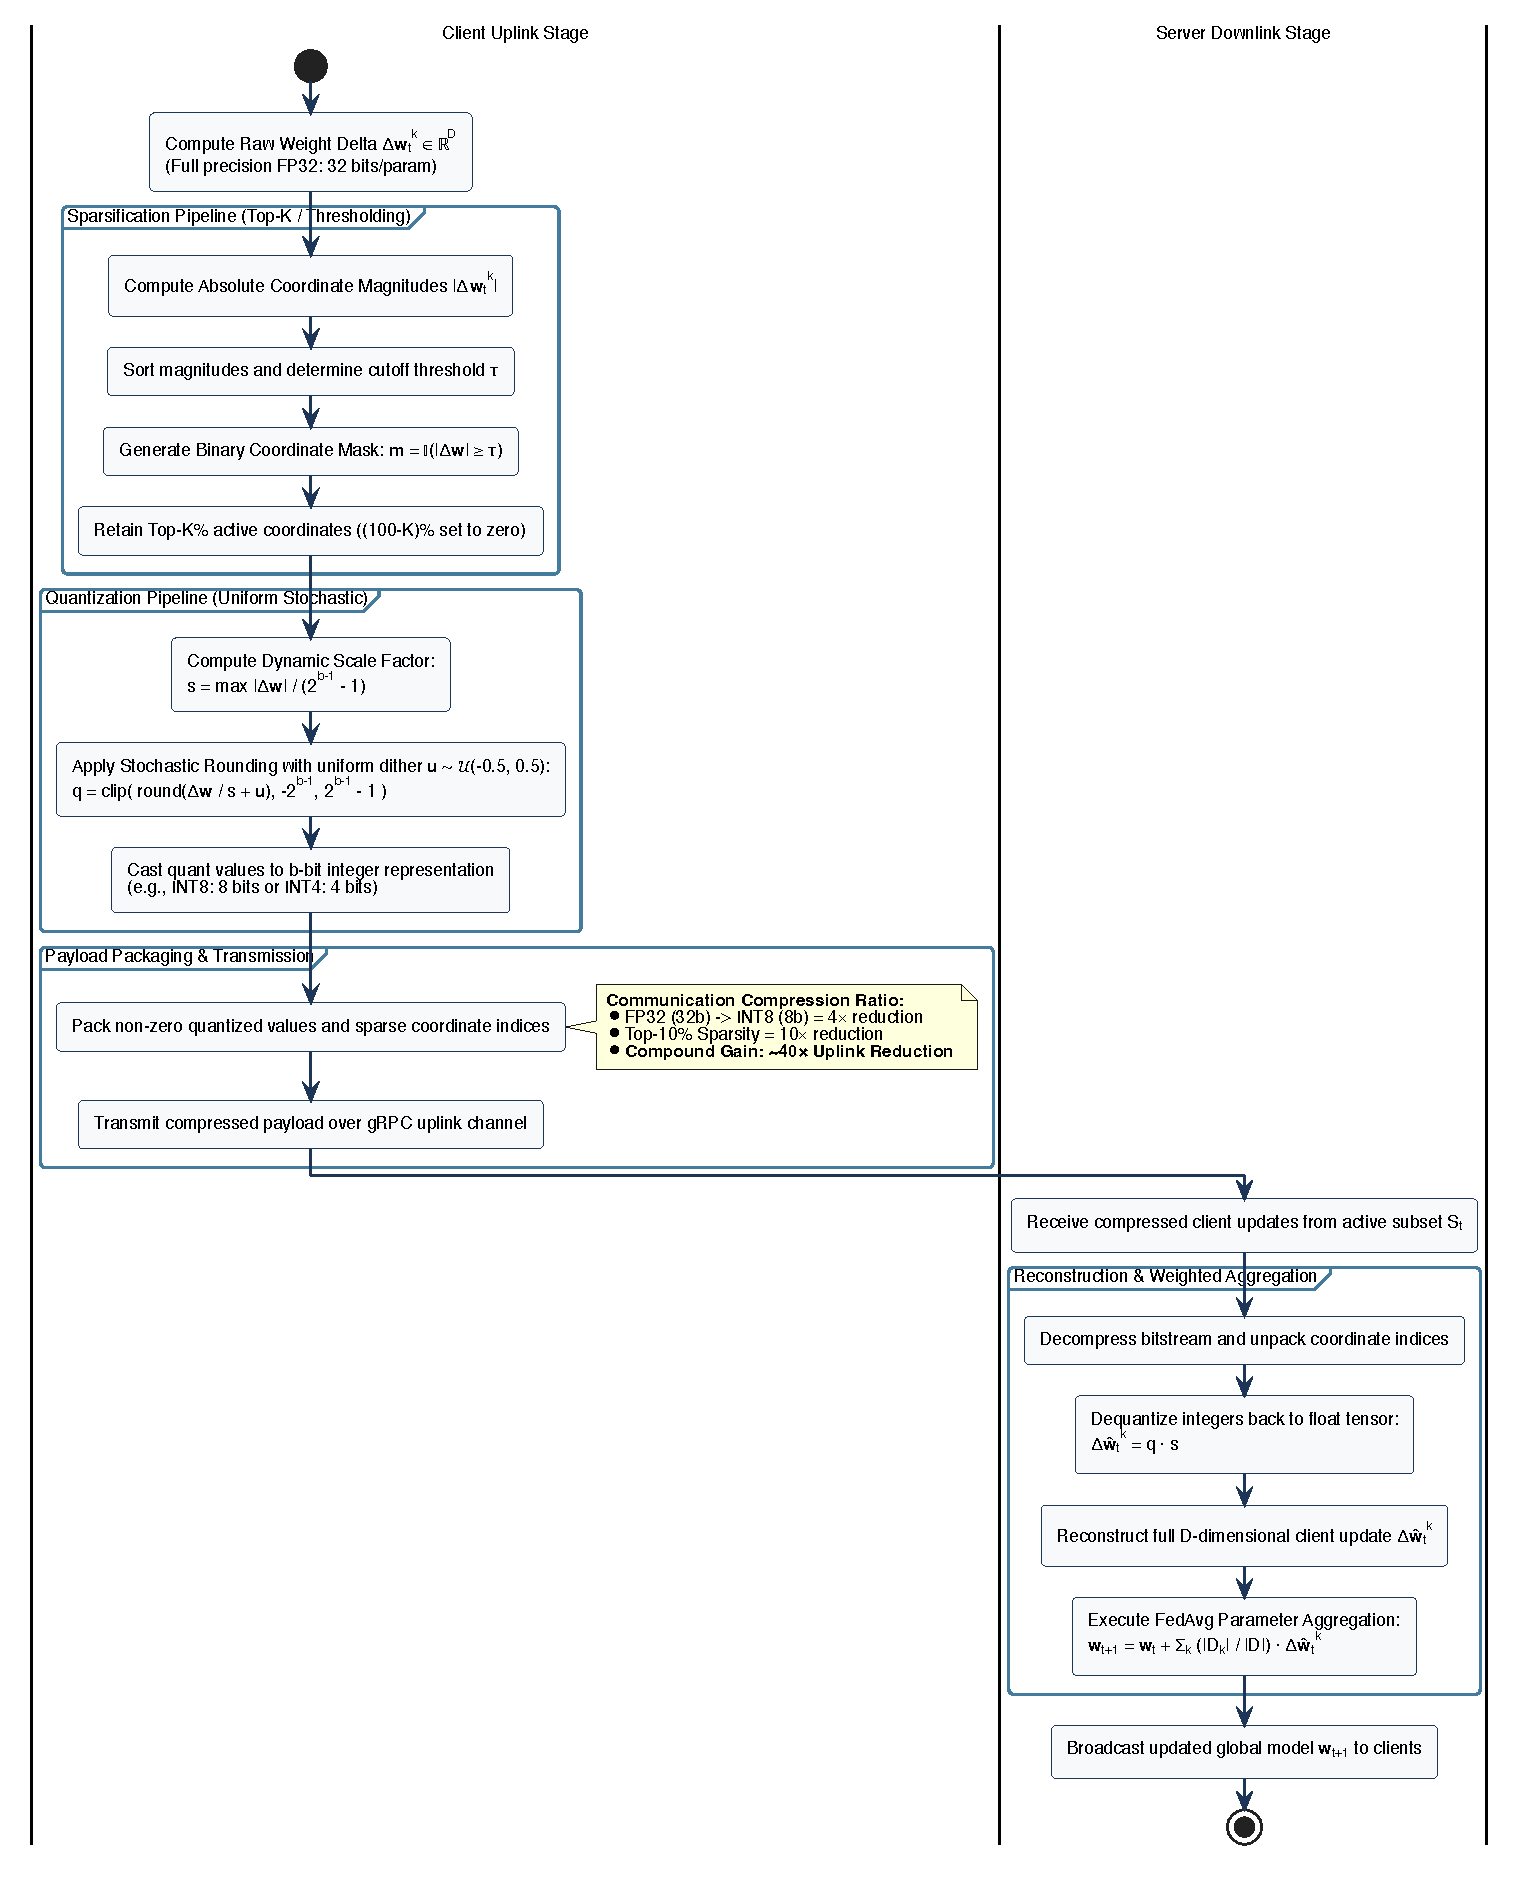
\includegraphics[width=\textwidth]{figures/communication_efficiency.pdf}
    \caption{Communication Efficiency Pipeline (\texttt{communication\_efficiency.svg}), detailing the swimlane pipeline for Top-$K$ sparsification, stochastic quantization, payload packing, and server-side reconstruction.}
    \label{fig:communication_efficiency}
\end{figure}

\section{Executive Summary \& Elevator Pitch}
\begin{elevatorpitch}
Communication bandwidth is the primary bottleneck in federated learning. Deep models such as ResNet-50 require transmitting over 100 megabytes per client round. Our communication efficiency pipeline combines two complementary techniques:
\begin{itemize}[leftmargin=*]
    \item \textbf{Top-$K$ Magnitude Sparsification}: Retains only the top $10\%$ most significant gradient coordinates ($10\times$ reduction).
    \item \textbf{Uniform INT8 Quantization}: Compresses 32-bit floats down to 8-bit signed integers ($4\times$ reduction).
\end{itemize}
Together, this compound compression delivers an overall \textbf{$\sim 40\times$ uplink bandwidth reduction} with minimal degradation in model accuracy.
\end{elevatorpitch}

\section{Pipeline Walkthrough: Client Uplink to Server Downlink}
\subsection{Client Uplink Stage}
\begin{enumerate}[leftmargin=*]
    \item \textbf{Raw Delta Computation}: Computes raw FP32 weight updates $\Delta\mathbf{w}_t^k \in \mathbb{R}^D$ (32 bits per parameter).
    \item \textbf{Top-$K$ Sparsification}: Computes absolute coordinate magnitudes $|\Delta w_j^k|$, determines cutoff threshold $\tau$, and constructs a binary selection mask $\mathbf{m} = \mathbb{I}(|\Delta w| \ge \tau)$. Coordinates below $\tau$ are set to zero.
    \item \textbf{Stochastic Uniform Quantization}: Evaluates dynamic scale factor $s = \frac{\max |\Delta w|}{2^{b-1} - 1}$, injects stochastic dither $u \sim \mathcal{U}(-0.5, 0.5)$, and clips rounded coordinates to signed $b$-bit integer bounds.
    \item \textbf{Bitstream Packaging}: Packs non-zero integer values and sparse coordinate indices into a compact payload, achieving a compound $\sim 40\times$ uplink reduction.
\end{enumerate}

\subsection{Server Downlink Stage}
\begin{enumerate}[leftmargin=*]
    \item \textbf{Unpacking \& Dequantization}: Extracts quantized integers $q$ and multiplies by scale factor $s$ to reconstruct approximate floating-point values $\Delta\hat{\mathbf{w}}_t^k = q \cdot s$.
    \item \textbf{Sparse Reconstruction}: Maps non-zero coordinates back to the full $D$-dimensional parameter space using the transmitted coordinate indices.
    \item \textbf{Weighted Aggregation}: Computes standard FedAvg aggregation over the reconstructed updates and broadcasts new global parameters $\mathbf{w}_{t+1}$.
\end{enumerate}

\section{Mathematical Formulations of Compound Compression}
\begin{mathfoundation}
\textbf{1. Top-$K$ Sparsification Operator}:
For vector $\mathbf{v} \in \mathbb{R}^D$ and sparsity ratio $\rho \in (0, 1]$ where $K = \lfloor \rho D \rfloor$:
\begin{equation}
    [\text{Top}_K(\mathbf{v})]_i = \begin{cases}
        v_i, & \text{if } |v_i| \ge |v_{(K)}| \\
        0, & \text{otherwise}
    \end{cases}
\end{equation}

\textbf{2. Uniform Stochastic Quantization}:
For bit-width $b$ (e.g., $b=8$), the scale factor and quantized values are defined as:
\begin{equation}
    s = \frac{\|\mathbf{v}\|_\infty}{2^{b-1} - 1}, \quad q_i = \text{clip}\left( \left\lfloor \frac{v_i}{s} + u_i \right\rceil, -2^{b-1}, 2^{b-1} - 1 \right)
\end{equation}
where $u_i \sim \mathcal{U}(-0.5, 0.5)$ ensures unbiased quantization:
\begin{equation}
    \mathbb{E}[q_i \cdot s \mid v_i] = v_i, \quad \mathbb{E}[\|\mathbf{v} - Q(\mathbf{v})\|_2^2] \le \frac{s^2 D}{4}
\end{equation}

\textbf{3. Error-Feedback SGD (EF-SGD) Formulation}:
To prevent gradient energy loss from biased Top-$K$ sparsification, uncommunicated residuals are accumulated in an on-device error memory buffer $\mathbf{e}_t^k$:
\begin{equation}
    \mathbf{p}_t^k = \mathbf{e}_t^k + \Delta\mathbf{w}_t^k, \quad \Delta\tilde{\mathbf{w}}_t^k = \text{Compress}(\mathbf{p}_t^k), \quad \mathbf{e}_{t+1}^k = \mathbf{p}_t^k - \Delta\tilde{\mathbf{w}}_t^k
\end{equation}
guaranteeing asymptotic convergence comparable to uncompressed FedAvg.
\end{mathfoundation}

\section{Compound Bandwidth Savings Analysis}
\begin{table}[htbp]
    \centering
    \small
    \caption{Uplink Communication Overhead per Client for ResNet-50 ($25.6 \times 10^6$ parameters)}
    \label{tab:bandwidth_comparison}
    \begin{tabular}{@{}lcccc@{}}
        \toprule
        \textbf{Compression Configuration} & \textbf{Bits/Param} & \textbf{Active Coords} & \textbf{Payload Size} & \textbf{Bandwidth Savings} \\
        \midrule
        Uncompressed Baseline (FP32) & 32 & 100\% & 102.4 MB & 1.0$\times$ (Baseline) \\
        INT8 Quantization Only & 8 & 100\% & 25.6 MB & 4.0$\times$ \\
        Top-10\% Sparsification Only & 32 & 10\% & 14.3 MB & 7.2$\times$ \\
        \textbf{Compound: Top-10\% + INT8} & \textbf{8} & \textbf{10\%} & \textbf{2.6 MB} & \textbf{39.4$\times$} \\
        \textbf{Compound: Top-5\% + INT4} & \textbf{4} & \textbf{5\%} & \textbf{0.8 MB} & \textbf{128.0$\times$} \\
        \bottomrule
    \end{tabular}
\end{table}

\section{Advisor Defense Questions \& Model Answers}
\begin{defenseqa}{Error-Feedback Compensation}
\textbf{Question}: \textit{"Why is Error Feedback (EF-SGD) mandatory when applying Top-$K$ sparsification, and what happens if you omit it?"}\\
\textbf{Answer}: Top-$K$ sparsification is a biased compression operator:
\begin{equation}
    \mathbb{E}[\text{Top}_K(\mathbf{v})] \ne \mathbf{v}
\end{equation}
Without error feedback, small gradient components that never exceed threshold $\tau$ are permanently discarded. Over successive rounds, these uncommunicated coordinates accumulate error, causing the model to diverge or plateau at suboptimal accuracy. With error feedback, dropped coordinates accumulate in memory buffer $\mathbf{e}_t^k$ until their aggregate magnitude exceeds $\tau$, ensuring all parameter updates are eventually communicated to the global model.
\end{defenseqa}

% ==============================================================================
% CHAPTER 9: COMPLETE MATHEMATICAL NOTATION & VARIABLE DICTIONARY
% ==============================================================================
\chapter{Mathematical Notation \& Variable Dictionary}
\label{chap:math_dictionary}

This chapter provides an exhaustive, symbol-by-symbol reference for every mathematical variable, operator, subscript, and Greek letter across the architecture.

\section{Federated Learning Foundations \& Aggregation}

\subsection{Global Objective Function}
\begin{equation}
    \min_{\mathbf{w} \in \mathbb{R}^D} F(\mathbf{w}) \triangleq \sum_{k=1}^K p_k F_k(\mathbf{w})
\end{equation}
\begin{itemize}[leftmargin=*]
    \item $\mathbf{w}$ (\textit{lowercase bold w}): The \textbf{model weight vector} (all trainable parameters: weights and biases flattened into a single list of numbers).
    \item $\mathbb{R}^D$: The \textbf{$D$-dimensional real space}. $D$ is the total parameter count (e.g., $D = 25.6 \times 10^6$ for ResNet-50).
    \item $\min_{\mathbf{w}}$: The \textbf{minimization operator}. We seek the specific configuration of weights $\mathbf{w}$ that minimizes the error function.
    \item $F(\mathbf{w})$: The \textbf{global objective function} (the average loss across all data in the entire federation).
    \item $\triangleq$: \textbf{Defined as}. Indicates that the left-hand side is formally defined by the right-hand side.
    \item $K$: The \textbf{total number of edge clients} in the network (e.g., $K = 100$ phones).
    \item $k$: The \textbf{client index} ($k \in \{1, 2, \dots, K\}$).
    \item $p_k$: The \textbf{aggregation weight} assigned to client $k$, representing client $k$'s proportion of the total data ($p_k \triangleq |D_k| / |D|$).
    \item $F_k(\mathbf{w})$: The \textbf{local empirical loss} evaluated exclusively on client $k$'s private dataset $D_k$.
\end{itemize}

\subsection{Local Client Loss Function}
\begin{equation}
    F_k(\mathbf{w}) \triangleq \frac{1}{|D_k|} \sum_{\xi \in D_k} \ell(\mathbf{w}; \xi)
\end{equation}
\begin{itemize}[leftmargin=*]
    \item $D_k$: The \textbf{private local dataset} stored strictly on client $k$'s edge hardware.
    \item $|D_k|$: The \textbf{cardinality (sample count)} of client $k$'s dataset (e.g., $|D_k| = 500$ images).
    \item $|D|$: The \textbf{total sample count} across all clients in the federation ($|D| = \sum_{k=1}^K |D_k|$).
    \item $\xi$: A single \textbf{data sample tuple} $(x, y)$, where $x$ is the input image tensor and $y$ is the ground-truth class label.
    \item $\ell(\mathbf{w}; \xi)$: The \textbf{per-sample loss function} (typically Cross-Entropy loss $\ell = -\log P(y \mid x; \mathbf{w})$).
\end{itemize}

\subsection{Parameter Deltas and Server Aggregation}
\begin{equation}
    \Delta\mathbf{w}_t^k \triangleq \mathbf{w}_{t, E}^k - \mathbf{w}_t, \quad \mathbf{w}_{t+1} = \mathbf{w}_t + \sum_{k \in S_t} \frac{|D_k|}{\sum_{j \in S_t} |D_j|} \Delta\mathbf{w}_t^k
\end{equation}
\begin{itemize}[leftmargin=*]
    \item $t$: The \textbf{current communication round number} ($t = 0, 1, 2, \dots$).
    \item $\mathbf{w}_t$: The \textbf{global model parameters} at the start of round $t$.
    \item $E$: The \textbf{number of local epochs} executed on each edge client per round.
    \item $\mathbf{w}_{t, E}^k$: The \textbf{local model parameters} of client $k$ after completing $E$ local training epochs starting from $\mathbf{w}_t$.
    \item $\Delta\mathbf{w}_t^k$ (\textit{Delta w}): The \textbf{parameter update delta} computed by client $k$. Represents how much client $k$ wants each parameter to change.
    \item $S_t$: The \textbf{sampled client cohort} selected by the server for round $t$ ($S_t \subseteq \{1, \dots, K\}$).
    \item $\mathbf{w}_{t+1}$: The \textbf{updated global model parameters} produced by server aggregation for the next round $t+1$.
\end{itemize}

\section{Data Heterogeneity \& Dirichlet Non-IID Partitioning}
\begin{equation}
    \mathbf{q}_c \sim \text{Dir}(\alpha \cdot \mathbf{1}_K), \quad P_k(Y = c) = \frac{q_{c, k} \cdot N_c}{\sum_{j=1}^C q_{j, k} \cdot N_j}
\end{equation}
\begin{itemize}[leftmargin=*]
    \item $C$: Total \textbf{number of target classes} (e.g., $C=10$ for CIFAR-10).
    \item $c$: Index of a \textbf{specific class} ($c \in \{1, \dots, C\}$).
    \item $\mathbf{q}_c$: A \textbf{probability distribution vector} of length $K$ defining the fraction of class $c$ assigned to each client.
    \item $\text{Dir}(\cdot)$: The \textbf{Dirichlet probability distribution}, a multivariate continuous distribution whose samples sum to 1.
    \item $\alpha$ (\textit{alpha}): The \textbf{concentration parameter}. Dictates data heterogeneity: $\alpha \to \infty$ produces balanced (IID) splits; $\alpha \le 0.1$ produces extreme non-IID label skew.
    \item $\mathbf{1}_K$: A vector of ones of length $K$ ($\mathbf{1}_K = [1, 1, \dots, 1]$), ensuring symmetric prior expectations across all clients.
    \item $q_{c, k}$: The scalar fraction of class $c$'s data allocated to client $k$.
    \item $N_c$: The total number of available samples belonging to class $c$ in the raw dataset.
    \item $P_k(Y = c)$: The \textbf{empirical probability} that a randomly drawn sample from client $k$ belongs to class $c$.
    \item $D_{\text{TV}}(P_k, P_j)$: The \textbf{Total Variation distance} between client $k$'s and client $j$'s label distributions, measuring discrepancy in $[0, 1]$.
\end{itemize}

\section{Optimization Algorithms: FedProx \& FedMuon}
\begin{equation}
    h_k(\mathbf{w}; \mathbf{w}_t) \triangleq F_k(\mathbf{w}) + \frac{\mu}{2} \|\mathbf{w} - \mathbf{w}_t\|_2^2
\end{equation}
\begin{itemize}[leftmargin=*]
    \item $h_k(\mathbf{w}; \mathbf{w}_t)$: The \textbf{regularized local objective function} used by FedProx on client $k$.
    \item $\mu$ (\textit{mu}): The \textbf{proximal regularization coefficient} ($\mu \ge 0$). Controls how strongly clients are penalized for moving too far from $\mathbf{w}_t$.
    \item $\|\mathbf{w} - \mathbf{w}_t\|_2^2$: The \textbf{squared Euclidean ($L_2$) distance} between local parameters $\mathbf{w}$ and global weights $\mathbf{w}_t$.
    \item $\mathbf{G}_t$: The \textbf{aggregated gradient direction} at the server: $\mathbf{G}_t = \sum p_k \Delta\mathbf{w}_t^k$.
    \item $\mathbf{M}_t$: The \textbf{momentum matrix buffer} in FedMuon: $\mathbf{M}_t = \beta \mathbf{M}_{t-1} + (1 - \beta) \mathbf{G}_t$.
    \item $\beta$ (\textit{beta}): The \textbf{momentum decay parameter} ($\beta \in [0, 1)$, typically $0.9$).
    \item $\text{Polar}(\mathbf{M}_t)$: The \textbf{polar decomposition operator}, which extracts the closest orthogonal matrix to $\mathbf{M}_t$ via iterative Newton-Schulz matrix updates.
\end{itemize}

\section{Differential Privacy via DP-SGD}
\begin{equation}
    \bar{\mathbf{g}}_i = \mathbf{g}_i \cdot \min\left(1, \frac{C}{\|\mathbf{g}_i\|_2}\right), \quad \tilde{\mathbf{g}} = \frac{1}{|B|} \left( \sum_{i=1}^{|B|} \bar{\mathbf{g}}_i + \mathcal{N}(0, \sigma^2 C^2 \mathbf{I}) \right)
\end{equation}
\begin{itemize}[leftmargin=*]
    \item $B$: The current \textbf{training mini-batch} of samples ($B \subset D_k$).
    \item $|B|$: The \textbf{mini-batch size} (e.g., $|B| = 32$).
    \item $i$: The \textbf{individual sample index} within mini-batch $B$ ($i \in \{1, \dots, |B|\}$).
    \item $\mathbf{g}_i$: The \textbf{unclipped per-sample gradient} $\nabla_{\mathbf{w}} \ell(\mathbf{w}; x_i, y_i)$ computed via \texttt{jax.vmap}.
    \item $\|\mathbf{g}_i\|_2$: The \textbf{Euclidean ($L_2$) norm} (geometric length) of gradient vector $\mathbf{g}_i$: $\sqrt{\sum_j g_{i, j}^2}$.
    \item $C$: The \textbf{clipping threshold} ($C > 0$). Caps the maximum sensitivity of any single sample's gradient.
    \item $\bar{\mathbf{g}}_i$: The \textbf{clipped gradient vector} for sample $i$, guaranteed to satisfy $\|\bar{\mathbf{g}}_i\|_2 \le C$.
    \item $\mathcal{N}(0, \sigma^2 C^2 \mathbf{I})$: A \textbf{multivariate Gaussian distribution} with zero mean and covariance $\sigma^2 C^2 \mathbf{I}$.
    \item $\sigma$ (\textit{sigma}): The \textbf{noise multiplier} (e.g., $\sigma = 1.0$). Higher $\sigma$ gives stronger privacy but lower accuracy.
    \item $\mathbf{I}$: The \textbf{identity matrix} of size $D \times D$, indicating that noise is added independently to every parameter.
    \item $\tilde{\mathbf{g}}$ (\textit{g-tilde}): The final \textbf{differentially private mini-batch gradient}.
    \item $\epsilon$ (\textit{epsilon}): The \textbf{privacy budget parameter}. Quantifies maximum information leakage. Lower $\epsilon$ indicates stronger privacy (e.g., $\epsilon \le 3.0$).
    \item $\delta$ (\textit{delta}): The \textbf{failure probability} that the $\epsilon$-DP guarantee fails (typically set to cryptographically tiny $\delta \le 10^{-5}$).
    \item $q$: The \textbf{Poisson subsampling ratio} $q \triangleq |B| / |D_k|$.
    \item $T$: The total \textbf{number of DP-SGD steps} executed across the training process.
\end{itemize}

\section{Communication Compression \& Error Feedback}
\begin{equation}
    s = \frac{\|\mathbf{v}\|_\infty}{2^{b-1} - 1}, \quad q_i = \text{clip}\left( \left\lfloor \frac{v_i}{s} + u_i \right\rceil, -2^{b-1}, 2^{b-1} - 1 \right)
\end{equation}
\begin{itemize}[leftmargin=*]
    \item $\mathbf{v}$: An arbitrary \textbf{parameter update vector} (e.g., $\Delta\mathbf{w}_t^k$).
    \item $v_i$: The $i$-th \textbf{scalar coordinate} of vector $\mathbf{v}$.
    \item $\|\mathbf{v}\|_\infty$: The \textbf{infinity norm} (maximum absolute value: $\max_j |v_j|$).
    \item $b$: The \textbf{target bit-width} for integer quantization (e.g., $b = 8$ for INT8, $b = 4$ for INT4).
    \item $2^{b-1} - 1$: The maximum positive integer representable in signed $b$-bit integer format ($127$ for INT8).
    \item $s$: The \textbf{dynamic quantization scale factor}. Maps continuous floats into discrete integer buckets.
    \item $u_i$: A \textbf{stochastic dither sample} drawn from continuous uniform distribution $\mathcal{U}(-0.5, 0.5)$, ensuring unbiased expectation $\mathbb{E}[q_i \cdot s] = v_i$.
    \item $\lfloor \cdot \rceil$: The \textbf{nearest integer rounding operator}.
    \item $q_i$: The resulting \textbf{$b$-bit integer} representing coordinate $v_i$.
    \item $\text{Top}_K(\mathbf{v})$: The \textbf{sparsification operator} that preserves only the $K$ largest magnitude coordinates and sets all others to 0.
    \item $\tau$ (\textit{tau}): The \textbf{magnitude cutoff threshold} below which coordinates are zeroed out.
    \item $\mathbf{e}_t^k$: The \textbf{error feedback memory buffer} on client $k$, which stores uncommunicated gradient residuals to prevent divergence.
\end{itemize}

\end{document}
